\documentclass[../main.tex]{subfiles}
\begin{document}
\chapter{Antagonism between substitutions in $\beta$-lactamase explains a path not taken in the evolution of bacterial drug resistance}
    \graphicspath{{Chapter2/}}
    \label{ch:chapter2}
    \captionsetup{labelfont=bf}

\textit{This chapter is adapted from the following publication:}

\textit{Brown, C.A., Hu, L., Sun, Z., Patel, M.P., Singh, S., Porter, J.R., Sankaran, B., Venkataram Prasad, B.V.V., Bowman, G.R., Palzkill, T., Antagonism between substitutions in $\beta$-lactamase explains a path not taken in the evolution of bacterial drug resistance, J.Biol., Chem., 2020, doi:10.1074/jbc.RA119.012489}\cite{brown_antagonism_2020}

\textit{My role in parameterizing and running molecular simulations of the crystal structures in apo and acyl-enzyme forms led to the data presented in figures \ref{fig:ch2-fig9} and \ref{fig:ch2-fig10}, and appendix figures \ref{fig:ch2-suppfig1}, \ref{fig:ch2-suppfig2}, \ref{fig:ch2-suppfig3}.}

    % \subsection{Contributions}
    %     My role in parameterizing and running molecular simulations of the crystal structures in apo and acyl-enzyme forms led to the data presented in figures \ref{fig:ch2-fig9} and \ref{fig:ch2-fig10}, and appendix figures \ref{fig:ch2-suppfig1}, \ref{fig:ch2-suppfig2}, \ref{fig:ch2-suppfig3}.   

    \section{Abstract}
        CTX-M $\beta$-lactamases are widespread in Gram-negative bacterial pathogens and provide resistance to the cephalosporin cefotaxime but not to the related antibiotic ceftazidime. Nevertheless, variants have emerged that confer resistance to ceftazidime. Two natural mutations, causing P167S and D240G substitutions in the CTX-M enzyme, result in 10-fold increased hydrolysis of ceftazidime. Although the combination of these mutations would be predicted to increase ceftazidime hydrolysis further, the P167S/D240G combination has not been observed in a naturally occurring CTX-M variant. Here, using recombinantly expressed enzymes, minimum inhibitory concentration measurements, steady-state enzyme kinetics, and X-ray crystallography, we show that the P167S/D240G double mutant enzyme exhibits decreased ceftazidime hydrolysis, lower thermostability, and decreased protein expression levels compared with each of the single mutants, indicating negative epistasis. X-ray structures of mutant enzymes with covalently trapped ceftazidime suggested that a change of an active-site $\Omega$-loop to an open conformation accommodates ceftazidime leading to enhanced catalysis. 10-$\mu$s molecular dynamics simulations further correlated Ω-loop opening with catalytic activity. We observed that the WT and P167S/D240G variant with acylated ceftazidime both favor a closed conformation not conducive for catalysis. In contrast, the single substitutions dramatically increased the probability of open conformations. We conclude that the antagonism is due to restricting the conformation of the Ω-loop. These results reveal the importance of conformational heterogeneity of active-site loops in controlling catalytic activity and directing evolutionary trajectories.

    
    \section{Introduction}
        Enzymes have evolved to catalyze reactions critical to the functioning of the cell\cite{knowles_enzyme_1991}. Evolution of enzyme function proceeds through the accumulation of amino acid substitutions that shape stability, solubility, and catalytic activity, among other properties. How substitutions interact when combined plays a key role in the trajectory of mutations that accumulate during evolution\cite{breen_epistasis_2012,de_visser_empirical_2014}. For example, amino acid substitutions can act additively on catalysis whereupon each substitution increases activity, and upon combination, the increase in activity in the double mutant is the product of the fold changes of the individual mutations\cite{wells_additivity_1990}. Alternatively, combinations of substitutions are often nonadditive where the double mutant has a greater activity or less activity than expected based on the activity of the single mutants. Such nonadditive effects are termed epistasis and can strongly influence the mutational pathways that are possible in the evolution of enzyme function\cite{weinreich_darwinian_2006}.

        Enzymes act by binding substrates and stabilizing transition states of reactions\cite{knowles_enzyme_1991}. Toward this end, conformational changes are often important, and flexible loops in the active site are a common feature involved in enzyme function\cite{dellus-gur_what_2013,doucet_flexibility_2009,whittier_conformational_2013}. Moreover, conformational dynamics have been proposed to play an important role in protein evolvability\cite{james_conformational_2003,tokuriki_protein_2009}. By this view, conformational fluctuations can result in an enzyme adopting multiple structures, some of which have properties that allow interactions with alternate ligands. These conformations may be rare in the ensemble of WT structures, but mutations may shift the distribution toward alternate conformations that become dominant in an evolved enzyme, thereby allowing for altered substrate specificity or new enzyme functions to emerge on an enzyme scaffold\cite{tokuriki_protein_2009,petrovic_conformational_2018}.

        Here, we address the role of epistasis and conformational diversity of active-site loops in the evolution of variants of the CTX-M $\beta$-lactamase with a broadened substrate specificity for $\beta$-lactam antibiotics. $\beta$-Lactams are the most frequently prescribed class of antibiotic worldwide, making up 65\% of all use\cite{livermore_-lactamase_2006}. However, bacterial resistance to these drugs is a growing problem, and the most common mechanism of resistance is enzyme-mediated hydrolysis of the $\beta$-lactam ring\cite{fisher_bacterial_2005}. This hydrolysis is catalyzed by various $\beta$-lactamases, which are divided into classes A–D based on primary amino acid sequence homology\cite{fisher_bacterial_2005,ambler_standard_1991}.

        Class A $\beta$-lactamases, such as CTX-M, are widespread in Gram-negative bacteria and share a similar mechanism of catalysis but can differ widely in substrate profile\cite{bush_epidemiological_2011,palzkill_structural_2018}. These enzymes are serine hydrolases that hydrolyze the amide bond in the $\beta$-lactam ring via sequential acylation and deacylation steps. The conserved catalytic Ser70 residue is activated by Lys73 and Glu166 for attack on the carbonyl carbon to form an acyl-enzyme intermediate. A catalytic water molecule is then activated by Glu166 for attack on the carbonyl of the covalent complex to deacylate the enzyme and release the product (Fig. \ref{fig:ch2-fig1})\cite{palzkill_structural_2018,mobashery_three_2009,bonomo_kinetics_2007}. The reaction scheme and mechanism of serine $\beta$-lactamases is shown in Fig. \ref{fig:ch2-fig1}.

        \begin{figure}[!htb] %Positioning code for figure
            \centering
            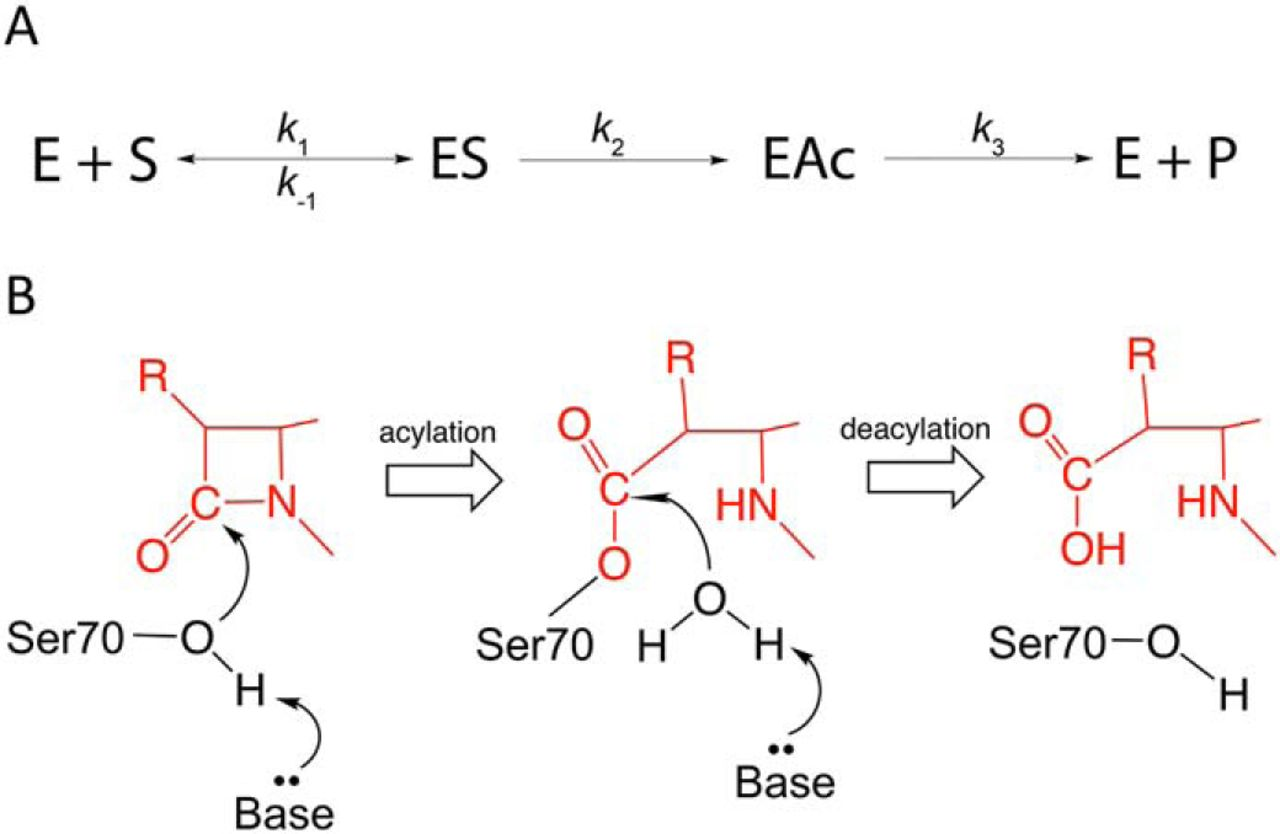
\includegraphics[width=3.5in]{ch2-fig1.jpg}
            \caption[$\beta$-Lactamase mechanism.]
                {$\beta$-Lactamase mechanism. A, reaction scheme for $\beta-$lactamase where E represents $\beta-$lactamase, ES represents the enzyme-substrate complex, EAc represents the acyl-enzyme complex, and P represents product. k1 and k-1 are the rate constants for association and dissociation of the enzyme substrate complex, and k2 and k3 are the rate constants for acylation and deacylation, respectively. B, schematic illustration of $\beta-$lactamase mechanism. The catalytic Ser70 hydroxyl group is activated for nucleophilic attack on the carbonyl oxygen of the amide bond of the $\beta-$lactam by an active-site residue serving as a general base. This residue is viewed as either Lys73 or Glu166 acting through a water molecule. This leads to formation of the acyl enzyme intermediate, which is subsequently deacylated by a water that is activated by Glu166 acting as a base and resulting in free enzyme and the hydrolyzed product.}
            \label{fig:ch2-fig1}
        \end{figure}

        CTX-M $\beta$-lactamases are a family of class A extended-spectrum $\beta$-lactamases that are so named because they efficiently hydrolyze the oxyimino-cephalosporin cefotaxime\cite{bonnet_growing_2004} (Fig. \ref{fig:ch2-fig2}). To date, more than 140 variants of the CTX-M enzymes have been identified\cite{dandrea_ctx-m-type_2013}. CTX-M-14 $\beta$-lactamase has become a model system for studies of the structure and function of CTX-M enzymes\cite{chen_atomic_2005,adamski_molecular_2015,patel_characterization_2015,patel_drug-resistant_2017}.

        \begin{figure}[!htb] %Positioning code for figure
            \centering
            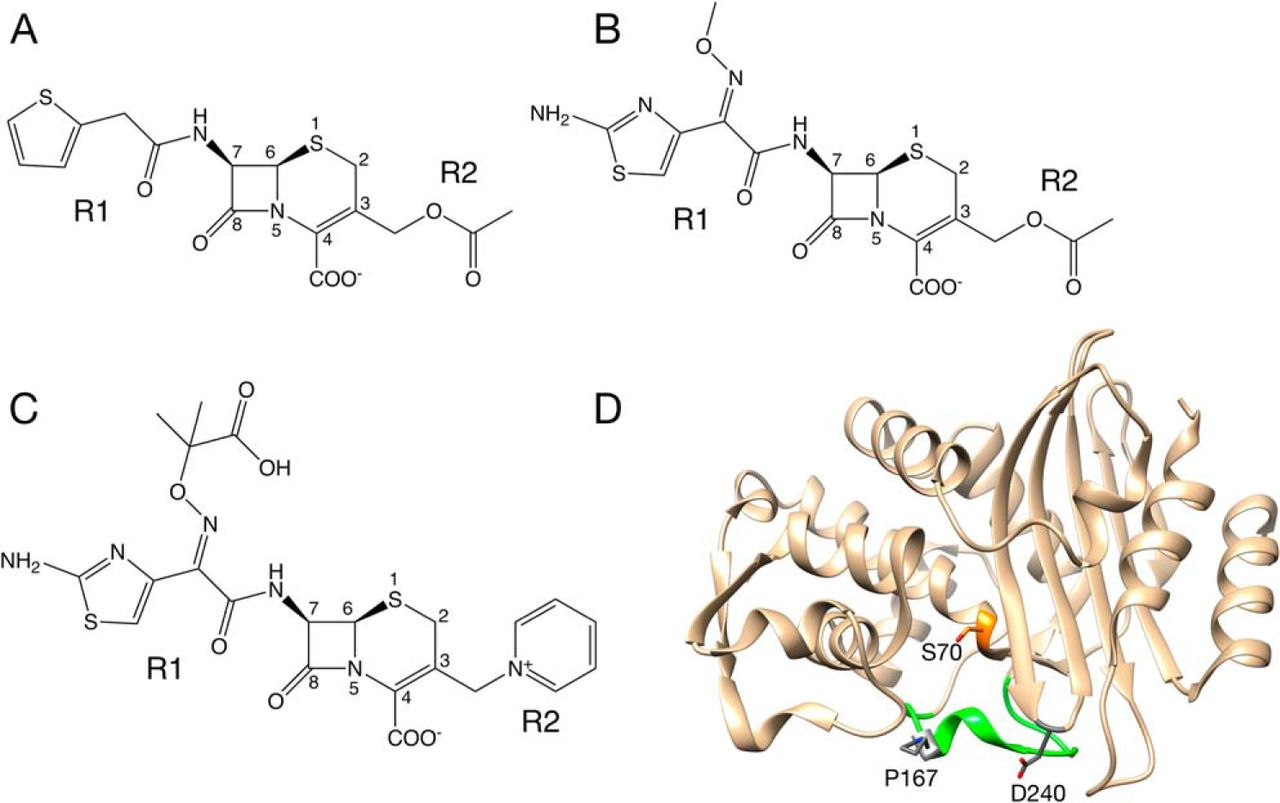
\includegraphics[width=3.5in]{ch2-fig2.jpg}
            \caption[Structures of antibiotics and CTX-M-14 $\beta$-lactamase.]
                {Structures of antibiotics and CTX-M-14 $\beta$-lactamase. A, cephalothin. R1 and R2 denote the groups that differ between cephalosporins. B, cefotaxime. C, ceftazidime. D, structure of CTX-M-14 $\beta$-lactamase (PDB code 1YLT). The $\Omega$-loop is colored green. The catalytic Ser70 is colored orange. Pro167 and Asp240 are colored gray. Note that Pro167 is located on the $\Omega$-loop.}
            \label{fig:ch2-fig2}
        \end{figure}

        CTX-M enzymes efficiently hydrolyze cefotaxime but not another commonly used oxyimino-cephalosporin, ceftazidime (Fig. \ref{fig:ch2-fig2}A). Natural variants containing either the P167S or D240G substitutions have emerged, however, that more efficiently hydrolyze ceftazidime\cite{dandrea_ctx-m-type_2013,bonnet_effect_2003,kimura_role_2004,canton_ctx-m_2012}. These two substitutions, when present, individually increase k$_{cat}$/K$_{m}$ for ceftazidime hydrolysis by 10-fold, resulting in increased ceftazidime resistance for bacteria containing the mutants\cite{chen_atomic_2005,patel_drug-resistant_2017}. Multiple natural variants in the CTX-M family possess one of these substitutions\cite{dandrea_ctx-m-type_2013}.

        Pro167 resides in the $\Omega$-loop that forms the bottom of the active site in class A $\beta$-lactamases including CTX-M enzymes\cite{chen_atomic_2005,strynadka_molecular_1992} (Fig. \ref{fig:ch2-fig2}D). It is adjacent to Glu166, which is conserved and serves as a general base to activate a water molecule for deacylation of $\beta$-lactam substrates\cite{strynadka_molecular_1992}. The peptide bond preceding Pro167 is in a cis conformation in CTX-M enzymes, which strongly influences the conformation of the $\Omega$-loop and the positioning of the Asn170 residue that hydrogen bonds to Glu166 and the deacylation water. We previously used the CTX-M-14 enzyme as a model system to examine the structural changes caused by the P167S substitution\cite{patel_drug-resistant_2017}. These studies revealed a large conformational change of the $\Omega$-loop that results in a larger active-site cavity to accommodate ceftazidime. This conformational change required both the P167S substitution and the presence of acylated ceftazidime\cite{patel_drug-resistant_2017} In addition, the structures showed that the conformational change is associated with a shift in the peptide bond preceding residue 167 from cis to trans and that the P167S substitution was required for this shift. Thus, the P167S substitution appears to cause increased ceftazidime hydrolysis through promoting a conformational change to relieve steric restraints on catalysis.

        Chen et al.\cite{chen_atomic_2005} previously determined the X-ray structure of the D240G mutant enzyme, and anisotropic B-factor analysis revealed increased flexibility of the B3 $\beta$-strand that forms one side of the CTX-M active site. The increased flexibility of the B3 $\beta$-stand was proposed to allow access for the bulky side chain of ceftazidime.

        Despite the increase in ceftazidime hydrolysis and bacterial resistance resulting from each of the substitutions, there has yet to be a CTX-M enzyme identified in clinical isolates that harbors both the P167S and D240G mutations. Based on simple additivity, the combination of substitutions that each increase hydrolysis by 10-fold would be expected to increased hydrolysis 100-fold relative to the WT enzyme\cite{wells_additivity_1990}. However, a P167S/D240G double mutant created by site-directed mutagenesis in a CTX-M-3 enzyme background exhibited a loss of ceftazidime resistance, indicating an antagonist effect and negative epistasis\cite{novais_mutational_2008}. The mechanism of this antagonism, however, was not examined.

        Here, we show that the P167S/D240G double mutant displays decreased ceftazidime hydrolysis compared with either of the single mutants, indicating antagonism. Further, X-ray structures of single and double mutants as apoenzymes and acylated with ceftazidime show alternate open and closed conformations of the $\Omega$-loop that are associated with high and low activity. Finally, molecular dynamics simulations of the WT, P167S, D240G, and P167S/D240G enzymes acylated with ceftazidime indicate that the single substitutions dramatically increase the probability of open conformations of the $\Omega$-loop, whereas the WT and P167S/D240G variant both favor a well-defined closed conformation not favorable for catalysis. Taken together, the results suggest that the P167S/D240G double mutant has not been observed in resistant clinical isolates because the combination results in decreased catalysis, decreased stability, and therefore decreased fitness in the presence of ceftazidime for bacteria containing this enzyme.

    
    \section{Results}
    \subsection{Ceftazidime resistance levels of P167S/D240G double mutant are reduced compared with single mutants.}

        The P167S and D240G substitutions have been observed in multiple CTX-M $\beta$-lactamase variants and are associated with 10-fold increased ceftazidime hydrolysis\cite{chen_atomic_2005,patel_characterization_2015}. Further, introduction of the P167S and D240G substitutions into the CTX-M-3 $\beta$-lactamase results in lower ceftazidime resistance than either of the single mutants\cite{novais_mutational_2008}. We extended these findings to the CTX-M-14 model system by determining minimum inhibitory concentrations (MICs)\ref{tab:ch2-tab1} for ceftazidime, cefotaxime, and cephalothin for Escherichia coli harboring WT and the mutants (Table \ref{tab:ch2-tab1}). The results show that the P167S and D240G individual substitutions both result in increased resistance to ceftazidime, whereas the P167S/D240G double mutant exhibits a loss of ceftazidime resistance compared with either the P167S or D240G single mutants (Table \ref{tab:ch2-tab1})\cite{patel_characterization_2015,novais_mutational_2008}. These data confirm the apparent incompatibility of the P167S and D240G substitutions as first suggested by Novais et al. \cite{novais_mutational_2008} and extends the findings to the CTX-M-14 enzyme background.

        \begin{table}[]
        \centering
        \caption[MICs for E. coli containing CTX-M-14 wild type, mutants, and no $\beta-$lactamase control]{MICs for E. coli containing CTX-M-14 wild type, mutants, and no $\beta-$lactamase control}
        \label{tab:ch2-tab1}
        \begin{tabular}{|l|l|l|l|}
        \hline
                    & \multicolumn{3}{l|}{MIC ($\mu$g/ml)}         \\ \hline
                    & Cephalothin       & Cefotaxime & Ceftazidime \\ \hline
        pTP123      & 12                & 0.0625     & 0.19        \\ \hline
        CTX-M-14 wt & \textgreater{}256 & 1.5        & 0.75        \\ \hline
        P167S       & \textgreater{}256 & 0.375      & 12          \\ \hline
        D240G       & \textgreater{}256 & 1          & 1.5         \\ \hline
        P167S/D240G & \textgreater{}256 & 0.19       & 0.75        \\ \hline
        \end{tabular}
        \end{table}

    \subsection{Antibiotic hydrolysis by the P167S/D240G double mutant is reduced compared with single mutants.}

        Although the P167S and D240G substitutions increase the catalytic efficiency (k$_{cat}$/K$_{m}$) for ceftazidime hydrolysis by $\sim$10-fold, the activity of the P167S/D240G double mutant enzyme has not been examined \cite{patel_characterization_2015,bonnet_effect_2003,kimura_role_2004,ishii_biochemical_2007}. Therefore, both WT and the double mutant CTX-M-14 enzymes were purified, and their kinetic parameters were determined for hydrolysis of the oxyimino-cephalosporins cefotaxime and ceftazidime, as well as cephalothin (Table \ref{tab:ch2-tab2}).

        \begin{table}[]
        \centering
        \caption[Enzyme kinetic parameters of CTX-M-14 $\beta$-lactamase and mutant enzymes]{Enzyme kinetic parameters of CTX-M-14 $\beta$-lactamase and mutant enzymes}
        \label{tab:ch2-tab2}
        \begin{tabular}{|l|l|l|l|l|}
        \hline
        Enzyme      & Parameter         & Cephalothin & Cefotaxime  & Ceftazidime       \\ \hline
        CTX-M-14    & k$_{cat}$ (s$^{-1}$)        & 1400 $\pm$ 38   & 161 $\pm$ 9     & NDa               \\\
                    & K$_{m}$ ($\mu$M)           & 83 $\pm$ 6      & 60 $\pm$ 7      & \textgreater{}500 \\
                    & k$_{cat}$/K$_{m}$ ($\mu$M$^{-1}$s$-1$) & 17.0 $\pm$ 0.7  & 2.71 $\pm$ 0.16 & 0.0011 $\pm$ 0.00007  \\ \hline
        P167Sb      & k$_{cat}$ (s$^{-1}$)        & 681 $\pm$ 36.8  & 297 $\pm$ 29.7  & ND                \\
                    & K$_{m}$ ($\mu$M)           & 32 $\pm$ 0.8    & 37 $\pm$ 6.3    & \textgreater{}500 \\
                    & k$_{cat}$/K$_{m}$ ($\mu$M$^{-1}$s$-1$) & 21.1 $\pm$ 1.3  & 8.0 $\pm$ 1.6   & 0.011 $\pm$ 0.0002    \\ \hline
        D240Gb      & k$_{cat}$ (s$^{-1}$)        & 471 $\pm$ 10.9  & 321 $\pm$ 46.2  & ND                \\
                    & K$_{m}$ ($\mu$M)           & 47.1 $\pm$ 41.7 & 52 $\pm$ 8.6    & \textgreater{}500 \\
                    & k$_{cat}$/K$_{m}$ ($\mu$M$^{-1}$s$-1$) & 10.0 $\pm$ 2.5  & 6.2 $\pm$ 1.4   & 0.013 $\pm$ 0.0007    \\ \hline
        P167S/D240G & k$_{cat}$ (s$^{-1}$)        & 165 $\pm$ 11    & 139 $\pm$ 3     & ND                \\
                    & K$_{m}$ ($\mu$M)           & 15 $\pm$ 3      & 42 $\pm$ 0.5    & \textgreater{}500 \\
                    & k$_{cat}$/K$_{m}$ ($\mu$M$^{-1}$s$-1$) & 10.8 $\pm$ 1.4  & 3.27 $\pm$ 0.1  & 0.0060 $\pm$ 0.00004 \\ \hline
        \end{tabular}
        \end{table}

        Ceftazidime hydrolysis by the WT, P167S, and D240G enzymes exhibits high K$_{m}$ values (>500 $\mu$M), which precluded determination of k$_{cat}$ values \cite{patel_characterization_2015}. Nevertheless, k$_{cat}$/K$_{m}$ values for the P167S and D240G enzymes were 10-fold higher than that observed for WT CTX-M-14. If the P167S and D240G substitutions act additively, k$_{cat}$/K$_{m}$ for ceftazidime by the double mutant should be a further 10-fold higher than that observed for the single mutants\cite{wells_additivity_1990}. However, k$_{cat}$/K$_{m}$ for ceftazidime hydrolysis by the double mutant was $\sim$2-fold lower than that observed for the P167S and D240G single mutants (Table \ref{tab:ch2-tab2}). Therefore, the P167S and D240G substitutions are antagonistic with respect to ceftazidime hydrolysis. This suggests that the presence of one substitution alters the environment of the other to perturb its contribution to catalysis\cite{wells_additivity_1990}.

        The P167S and D240G substitutions were previously observed to modestly increase k$_{cat}$/K$_{m}$ for cefotaxime hydrolysis ($\sim$2-fold) compared with the WT enzyme\cite{patel_characterization_2015}. The P167S/D240G double mutant exhibited a k$_{cat}$/K$_{m}$ value similar to WT and 2-fold lower than the single mutants indicating possible antagonism, as found for ceftazidime hydrolysis (Table \ref{tab:ch2-tab2}).

        The second-generation cephalosporin cephalothin is an excellent substrate for the WT CTX-M-14 enzyme (Table \ref{tab:ch2-tab2})\cite{patel_characterization_2015}. The P167S and D240G substitutions reduce both k$_{cat}$ and K$_{m}$ values for cephalothin hydrolysis (Table \ref{tab:ch2-tab2}). The P167S/D240G double mutant exhibited a further reduction in k$_{cat}$ and K$_{m}$ compared with the single mutants. Interestingly, the P167S and D240G substitutions act additively in the double mutant for cephalothin hydrolysis. Therefore, the additivity relationship between the P167S and D240G substitutions is substrate-dependent, with simple additivity observed for cephalothin and antagonism observed for ceftazidime hydrolysis, suggesting that the effects are mediated through interaction with the substrates.

    \subsection{P167S/D240G double mutant exhibits reduced stability compared with single mutants}

        Amino acid substitutions can affect catalysis, as shown above, but also can impact protein stability. It was previously shown that the P167S and D240G single mutants destabilize CTX-M-14\cite{patel_characterization_2015}. We extended this finding to the P167S/D240G enzyme using CD spectroscopy to monitor $\alpha$-helix ellipticity with increasing temperature (Fig. \ref{fig:ch2-fig3}). Previous studies showed that the WT CTX-M-14 exhibited a melting temperature (Tm) of 54.6 °C, and the single mutants D240G and P167S decreased the Tm by 0.4 and 2.8 °C, respectively\cite{patel_characterization_2015}. The P167S/D240G enzyme exhibited a Tm of 50.5 °C, indicating that the double mutant is less stable than WT and the single mutants (Fig. \ref{fig:ch2-fig3}).

        \begin{figure}[!htb] %Positioning code for figure
            \centering
            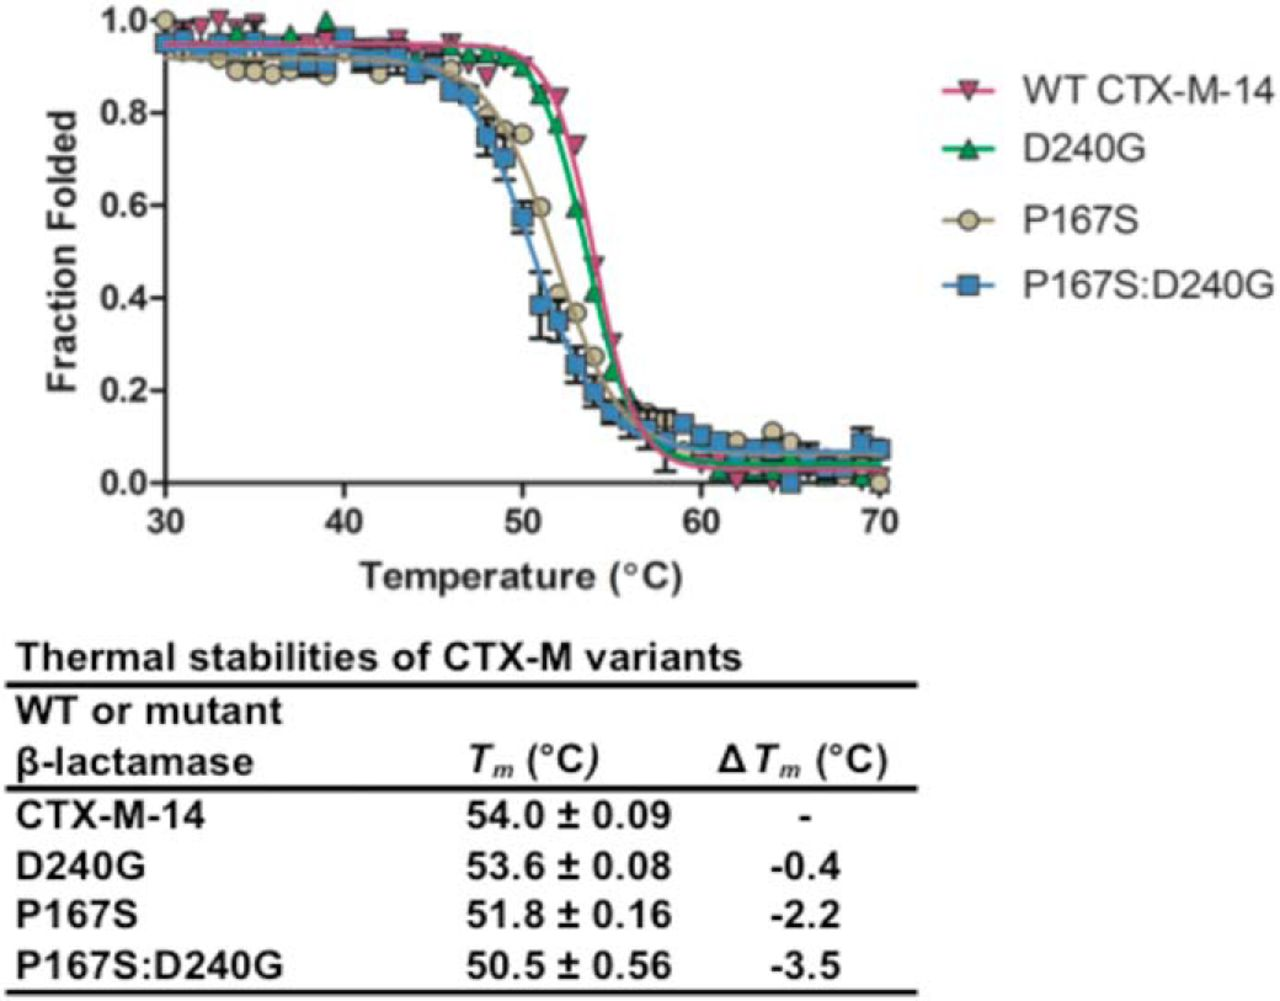
\includegraphics[width=3in]{ch2-fig3.jpg}
            \caption[Thermal stability of WT and mutant $\beta$-lactamases, as measured by CD.]
                {Thermal stability of WT and mutant $\beta$-lactamases, as measured by CD. Mean ellipsivity is normalized and fit to a Boltzmann sigmoidal function. Tm, as determined by the Boltzmann equation, is also plotted, as is $\Delta$Tm, which is the change from the WT Tm. The Tm indicates that each single mutant is less stable than the WT CTX-M-14 enzyme, and this instability has an additive effect in the double mutant, P167S/D240G CTX-M-14. The data for CTX-M-14, D240G, and P167S are from Patel et al.\cite{patel_characterization_2015}.}
            \label{fig:ch2-fig3}
        \end{figure}

    \subsection{Steady-state levels of the P167S/D240G enzyme in E. coli are reduced compared with single mutants.}

        The level of antibiotic resistance conferred to bacteria by a $\beta$-lactamase depends on the rate of hydrolysis, as well as the steady-state levels of enzyme expression\cite{huang_natural_1997}. A correlation has been shown between $\beta$-lactamase stability and expression levels in E. coli caused by increased proteolysis and aggregation of unstable proteins\cite{huang_natural_1997,brown_multiple_2010,mayer_correlation_2007}. Because the P167S and D240G substitutions decrease enzyme stability and the double mutant decreases stability further, we hypothesized that the double mutant would display lower expression levels. Immunoblot analysis of whole cell lysates using $\alpha$-CTX-M-14 $\beta$-lactamase polyclonal antibody showed that the P167S mutant did not significantly decrease expression levels relative to WT, consistent with previous studies (Fig. \ref{fig:ch2-fig4})\cite{patel_characterization_2015}. The D240G mutant, which shows only a 0.4 °C decrease in stability relative to WT, displayed lower expression levels. Thus, although D240G has higher thermal stability than P167S, it displays lower expression levels, indicating that thermal stability does not fully correlate with expression levels. However, the P167S/D240G enzyme exhibited lower expression levels than either WT or the P167S and D240G single mutants, consistent with the lower thermal stability of this mutant. Taken together, these findings provide a rationale for why the P167S/D240G double mutant has not been observed in resistant clinical isolates in that it is compromised for catalysis, stability, and expression levels compared with the P167S and D240G single mutants.

        \begin{figure}[!htb] %Positioning code for figure
            \centering
            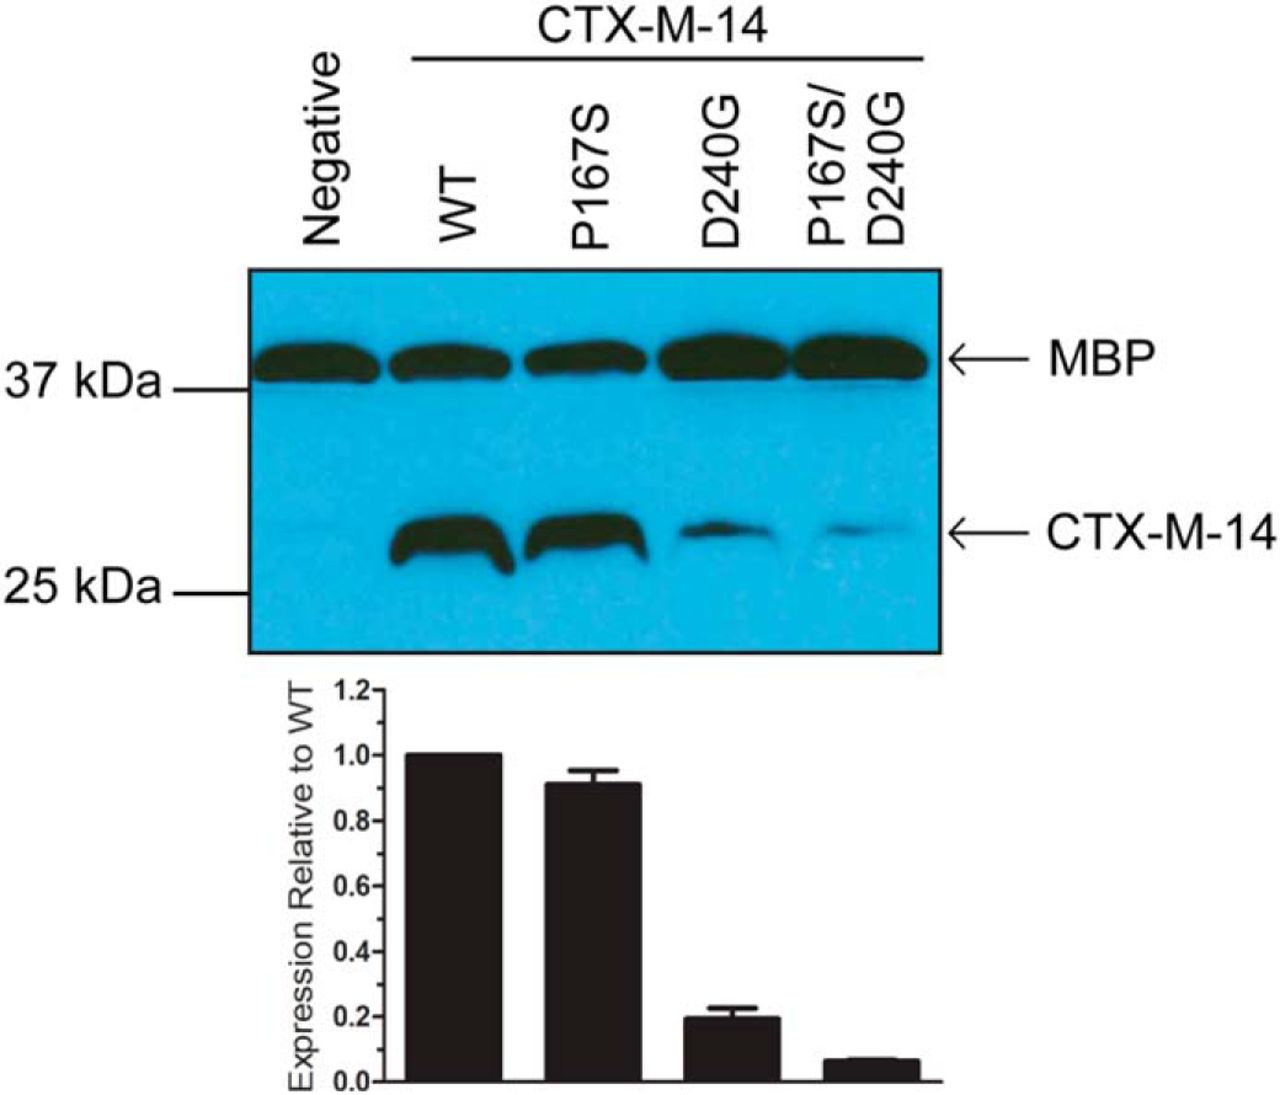
\includegraphics[width=3in]{ch2-fig4.jpg}
            \caption[Steady-state protein levels of WT CTX-M-14 and mutant $\beta$-lactamases.]
                {Steady-state protein levels of WT CTX-M-14 and mutant $\beta$-lactamases. Western blotting analysis with an anti-CTX-M-14 polyclonal antibody shows protein expression levels of WT CTX-M-14 and the P167S, D240G, and P167S/D240G mutants in the periplasm of recombinant E. coli cells. Analysis with a polyclonal antibody to the periplasmic protein MBP was used as a loading control. The hybridization signal was visualized by chemiluminescence and quantified by densitometry. The signal for CTX-M-14 $\beta$-lactamase was normalized to that for MBP in the same sample. The protein levels of mutant CTX-M-14 $\beta$-lactamase are expressed relative to that of WT CTX-M-14 $\beta$-lactamase in the bar graph. The quantification data in the bar graph are the averages of two independent experiments, and one representative immunoblot result is shown above the bar graph.}
            \label{fig:ch2-fig4}
        \end{figure}

    \subsection{X-ray structures of P167S/D240G apo, E166A/D240G/CAZ, and E166A/P167S/D240G/CAZ acyl-enzyme complexes reveal alternate conformations of the $\Omega$-loop.}

        We previously determined the X-ray structure of the P167S enzyme, which had a very similar overall structure as WT \cite{patel_drug-resistant_2017}. The $\Omega$-loop, which forms the bottom of the active site, was in a folded, closed conformation with the peptide bond preceding Ser167 in a cis configuration (Fig. \ref{fig:ch2-fig5}, A–C). The structure of the D240G enzyme was previously determined, and it also is highly similar to the WT structure\cite{chen_atomic_2005} (Fig. \ref{fig:ch2-fig5}D). We next determined the structure of the P167S/D240G enzyme, which exhibits lower ceftazidime hydrolysis than either of the single mutants. The structure includes a boronic acid from the crystallization buffer in complex with Ser70 and is very similar to the WT, P167S, and D240G structures, with the Ser167 peptide bond in the cis configuration and the $\Omega$-loop in a folded, closed conformation (Fig. \ref{fig:ch2-fig5}, E–H, and Table \ref{tab:ch2-supptable1}). A difference was noted, however, in the B-factors in the active-site 103–106 loop, suggesting increased disorder. B-factors reflect the degree to which electron density is scattered and therefore indicate how ordered an atom is in the structure\cite{yuan_prediction_2005}. The B-factors for residues in the 103–106 loop and the 164–179 $\Omega$-loop were normalized to the overall B-factor of each structure to facilitate comparison across structures (Fig. \ref{fig:ch2-fig6}). The normalized B-factors for the P167S/D240G structure for residues Val103 and Asn104 were higher than in the WT, P167S, and D240G structures. These findings suggest increased disorder for residues 103–104 in the P167S/D240G structure. We have previously shown that Asn104 is important for cefotaxime and ceftazidime hydrolysis, and therefore increased disorder of this residue in the P167S/D240G enzyme could result in the observed lower activity for ceftazidime hydrolysis\cite{patel_synergistic_2018}.

        \begin{figure}[!htb] %Positioning code for figure
            \centering
            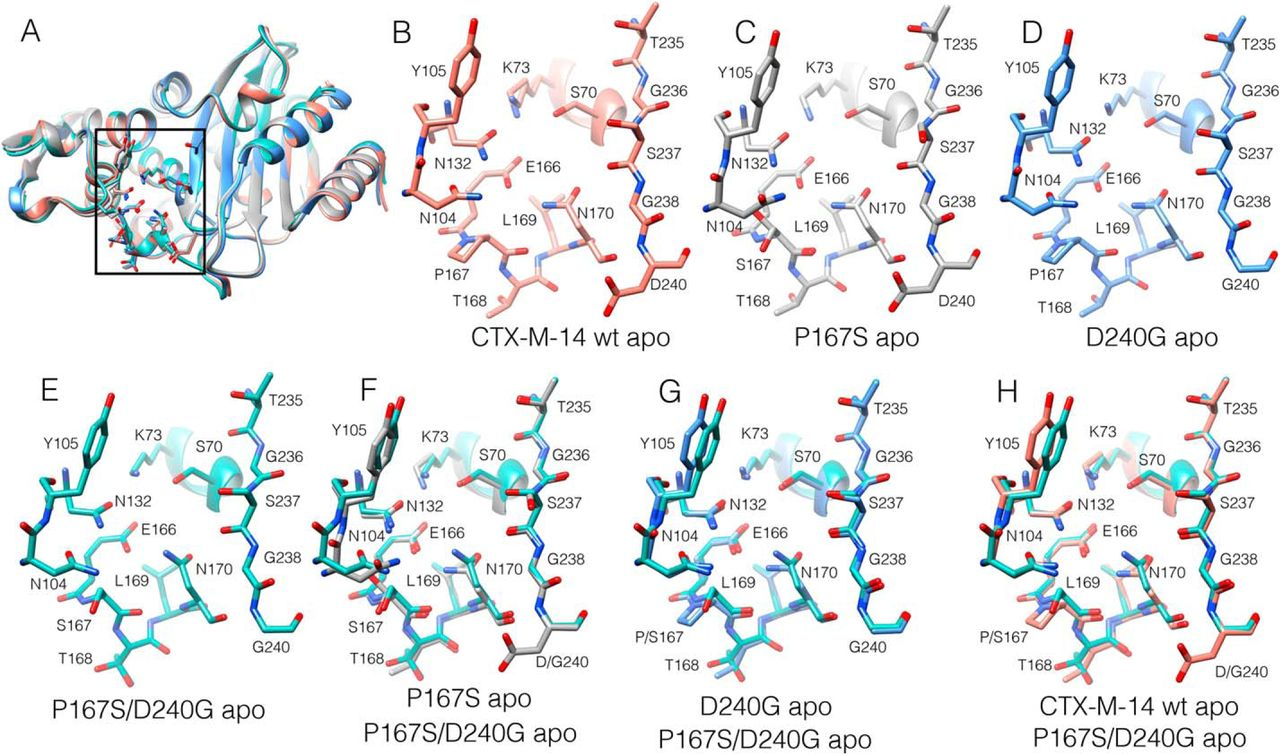
\includegraphics[width=5in]{ch2-fig5.jpg}
            \caption[Structures of the active-site region of WT CTX-M14 $\beta$-lactamase, as well as P167S, D240G, and P167S/D240G mutant enzymes in the apo form.]
                {Structures of the active-site region of WT CTX-M14 $\beta$-lactamase (PDB code 1YLT), as well as P167S (PDB code 5TWD), D240G (PDB code 1YLP), and P167S/D240G mutant enzymes in the apo form. A, ribbon diagram showing structural alignment of the CTX-M-14 WT (salmon), P167S (gray), D240G (blue), and P167S/D240G (cyan) enzymes. The active-site region shown in B–H is boxed. B–E, active-site regions of CTX-M-14 WT (B), P167S (C), D240G (D), and P167S/D240G (E). Note that the P167S/D240G structure has a boronic acid in complex with Ser70, which is not shown for clarity. F, structural alignment of active-site region of P167S apo enzyme (gray) with the P167S/D240G double mutant (cyan). G, structural alignment of D240G apo enzyme (blue) with P167S/D240G (cyan). H, structural alignment of CTX-M-14 WT apo enzyme with P167S/D240G (cyan). In all panels, oxygen is shown in red, and nitrogen is in blue.}
            \label{fig:ch2-fig5}
        \end{figure}

        We next determined the structures of the mutant enzymes in complex with ceftazidime to evaluate whether the presence of substrate influences active-site structure (Table \ref{tab:ch2-supptable1}). The E166A mutation blocks deacylation and allows for crystallization of the acyl-enzyme complex\cite{strynadka_molecular_1992}. The previously determined structure of the acyl-enzyme complex of the CTX-M-14 pseudo WT E166A enzyme with ceftazidime (E166A/CAZ) shows the Pro167 peptide bond in the cis configuration and the $\Omega$-loop in the folded, closed conformation (Fig. \ref{fig:ch2-fig7}A) \cite{patel_drug-resistant_2017}. Contacts between ceftazidime and the enzyme include hydrogen bonds between the side chains of Asn132 and Asn104 with the carbonyl oxygen of the acylamide of the ceftazidime R-2 group, as well as hydrogen bonds between the hydroxyls of Thr235 and Ser237 with the C4 carboxylate of the dihydrothiazine ring (Figs. \ref{fig:ch2-fig2}C and \ref{fig:ch2-fig7}A). The imino group of ceftazidime is pointed to solvent and does not interact with the enzyme. The previously determined structure of E166A/P167S/CAZ (Fig. 7B) shows the Ser167 peptide bond in the trans configuration and the $\Omega$-loop in an unraveled, open conformation, which widens the floor of the active site by $\sim$5 \AA{} to accommodate ceftazidime\cite{patel_drug-resistant_2017}. This leads to a change in conformation of ceftazidime in the acyl-enzyme with the aminothiazole ring assuming a buried position (Fig. \ref{fig:ch2-fig7}B)\cite{patel_drug-resistant_2017}. In addition, there are hydrogen bonds between the C4 carboxylate of the dihydrothiazine ring and the side chains of Thr235 and Ser237, as well as between the side chains of Asn132 and Asn104 with the carbonyl oxygen of the acylamide group (Fig. \ref{fig:ch2-fig7}B). Further, there is a hydrogen bond between Asn104 and the carboxyl group of the imino side chain of ceftazidime. These interactions are consistent with tighter binding of ceftazidime and enhanced catalysis\cite{patel_drug-resistant_2017}. In addition, the normalized B-factors of Val103 and Asn104 are not increased relative to WT CTX-M-14, suggesting that the Asn104 residue is well-ordered for interaction with ceftazidime (Fig. \ref{fig:ch2-fig6}A). Residues 168–170, however, show elevated B-factors, suggesting that the $\Omega$-loop has increased flexibility, consistent with its unfolded structure (Fig. \ref{fig:ch2-fig6}B).

        \begin{figure}[!htb] %Positioning code for figure
            \centering
            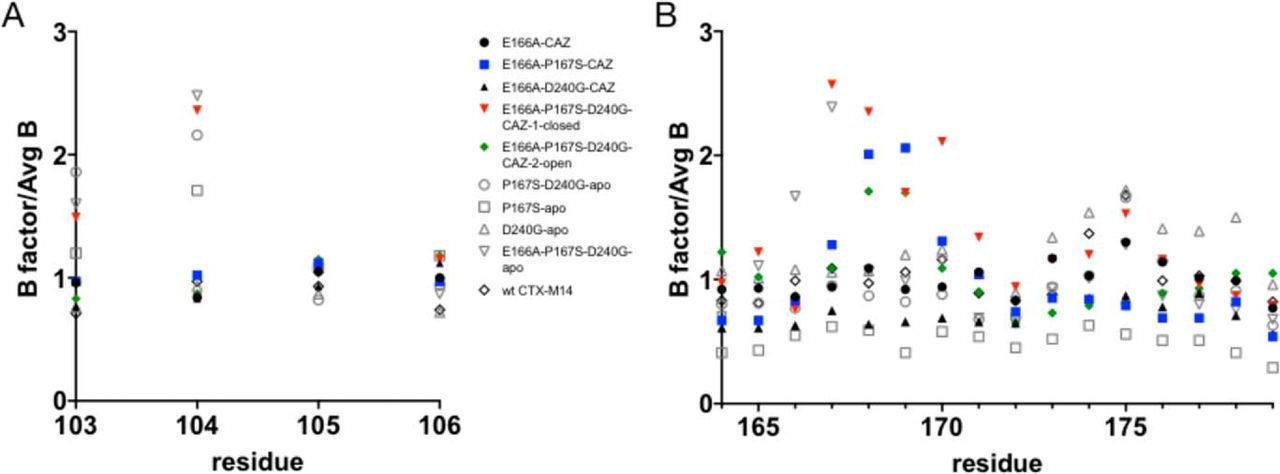
\includegraphics[width=4.7in]{ch2-fig6.jpg}
            \caption[Normalized B-factors for the 103–106 loop and the 164–179 $\Omega$-loop in the CTX-M enzyme structures.]
                {Normalized B-factors for the 103–106 loop and the 164–179 $\Omega$-loop in the CTX-M enzyme structures. The B-factors were normalized by dividing the B-factor for a given residue by the average B-factor for the entire structure. Thus, a normalized B-factor of 1 means the B-factor at that residue is the same as the average B-factor of the structure. A, normalized B-factors for the 103–106 loop. B, normalized B-factors for the 164–179 $\Omega$-loop. Black circle, E166A/CAZ; blue square, E166A/P167S/CAZ; black triangle, E166A/D240G/CAZ; inverted red triangle, E166A/P167S/D240G/CAZ-1; green diamond, E166A/P167S/D240G/CAZ-2; open circle, P167S/D240G apo; open square, P167S apo; open triangle, D240G apo; inverted open triangle, E166A/P167S/D240G apo; open diamond, CTX-M-14 WT.}
            \label{fig:ch2-fig6}
        \end{figure}

        The D240G substitution is also associated with increased ceftazidime hydrolysis\cite{bonnet_effect_2003,canton_ctx-m_2012}. We therefore determined the structure of the E166A/D240G enzyme in complex with ceftazidime for comparison with the E166A and E166A/P167S acyl-enzyme structures. It was found that the peptide bond preceding Pro167 is in the cis configuration, and the $\Omega$-loop is in the folded, closed conformation similar to the D240G apo enzyme structure and the E166A structure with ceftazidime (Fig. \ref{fig:ch2-fig7}C). In contrast to the E166A/CAZ structure, however, the E166A/D240G/CAZ structure has the side chain of Ser237 rotated away from the C4 carboxylate and instead forms hydrogen bonds to the carboxylate of the imino side chain, which may facilitate substrate binding and catalysis (Figs. \ref{fig:ch2-fig2}C and \ref{fig:ch2-fig7}C).

        \begin{figure}[!htb] %Positioning code for figure
            \centering
            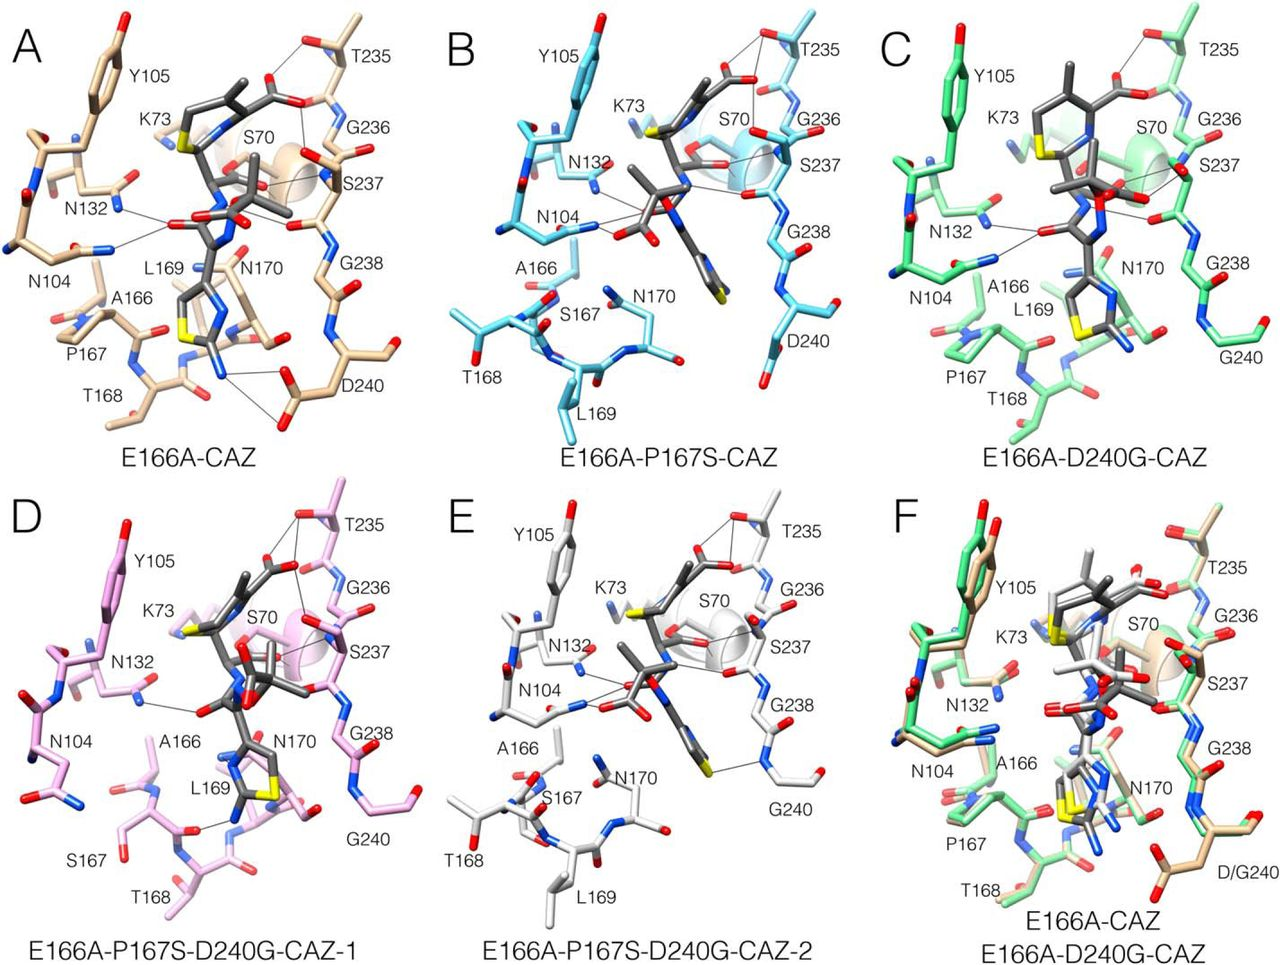
\includegraphics[width=4.7in]{ch2-fig7.jpg}
            \caption[Structures of the active-site region of CTX-M-14 mutant $\beta$-lactamase acyl-enzyme complexes with ceftazidime.]
                {Structures of the active-site region of CTX-M-14 mutant $\beta$-lactamase acyl-enzyme complexes with ceftazidime. A, structure of the E166A mutant (tan) with ceftazidime (dark gray) trapped in the acyl-enzyme form (PDB code 5U53). Oxygen is shown in red, and nitrogen is in blue. Hydrogen bonds are indicated by thin black lines. Active-site residues are labeled. B, structure of the E166A/P167S/CAZ acyl-enzyme (light blue) (PDB code 5TW6). C, structure of the E166A/D240G/CAZ acyl-enzyme (light green). D, structure of the E166A/P167S/D240G/CAZ-1 acyl-enzyme (pink). E, structure of the E166A/P167S/D240G/CAZ-2 acyl-enzyme (white). F, structural alignment of the E166A/CAZ (tan) and E166A/D240G/CAZ (green) acyl-enzyme complexes. The ceftazidime from the E166A/CAZ structure is shown in dark gray, and that from E166A/D240G/CAZ is shown in white. The $\Omega$-loop region remains folded in the closed form and the ceftazidime occupies a similar position with the aminothiazole ring surface exposed in these structures.}
            \label{fig:ch2-fig7}
        \end{figure}

        The P167S/D240G enzyme displays lower catalytic activity toward ceftazidime than either single mutant (Table \ref{tab:ch2-tab2}). To better understand the basis of this antagonism, we determined the structure of the E166A/P167S/D240G enzyme in complex with ceftazidime. Two structures from different space groups were obtained, and interestingly, they show different conformations of ceftazidime and the $\Omega$-loop. In the first structure, the peptide bond preceding Ser167 is in the trans configuration, which is in contrast to the cis bond found in the P167S/D240G apo structure (Fig. \ref{fig:ch2-fig5}, D and E). However, the $\Omega$-loop in the E166A/P167S/D240G/CAZ-1 structure remains in the folded, closed conformation with ceftazidime located in a similar position as that in the E166A/D240G/CAZ structure (Fig. \ref{fig:ch2-fig7}D). There are differences, however, between these structures. First, the carboxylate group of the imino side chain of ceftazidime in the E166A/P167S/D240G/CAZ-1 structure does not contact the enzyme, in contrast to the E166A/D240G/CAZ structure (Fig. \ref{fig:ch2-fig7}, C and D). More importantly, the positioning of the active-site 103–106 loop is altered, and the side chain of Asn104 is shifted out of the active site in the E166A/P167S/D240G/CAZ-1 structure (Fig. \ref{fig:ch2-fig7}D). In addition, the normalized B-factors for residues Val103 and Asn104 are elevated compared with the E166A/CAZ, E166A/P167S/CAZ, and E166A/D240G/CAZ structures, suggesting that Val103 and Asn104 are disordered (Fig. \ref{fig:ch2-fig6}A). We have previously shown that the hydrogen bond between Asn104 and the acyl-amide of cefotaxime and ceftazidime is important, and a N104A mutant exhibits 10-fold lower k$_{cat}$/K$_{m}$ for both substrates\cite{patel_synergistic_2018}. These observations suggest that the conformation of the enzyme and ceftazidime observed in the E166A/P167S/D240G/CAZ-1 structure is not consistent with hydrolysis.

        It is noteworthy that the E166A/P167S/D240G/CAZ-1 structure described above was obtained by soaking a crystal with ceftazidime. Another crystal was also soaked, and the structure was determined with the same space group, but ceftazidime was not present in the active site. Interestingly, this apo structure is very similar to the structure with bound ceftazidime. The peptide bond preceding Ser167 is in the trans configuration and the $\Omega$-loop is in the folded, closed conformation (Fig. \ref{fig:ch2-fig8}, C and D). In addition, the 103–106 loop is in a similar position as in the ceftazidime-bound structure with the side chain of Asn104 pointed out of the active site and with elevated B-factors for Val103 and Asn104 (Fig. \ref{fig:ch2-fig6}A). Thus, this conformation of the enzyme, and particularly the 103–106 loop, occurs in the absence of ceftazidime, in contrast to the different conformations of the E166A/P167S apo and E166A/P167S/CAZ structures where the presence of ceftazidime is apparently required to produce the conformational change.

        \begin{figure}[!htb] %Positioning code for figure
            \centering
            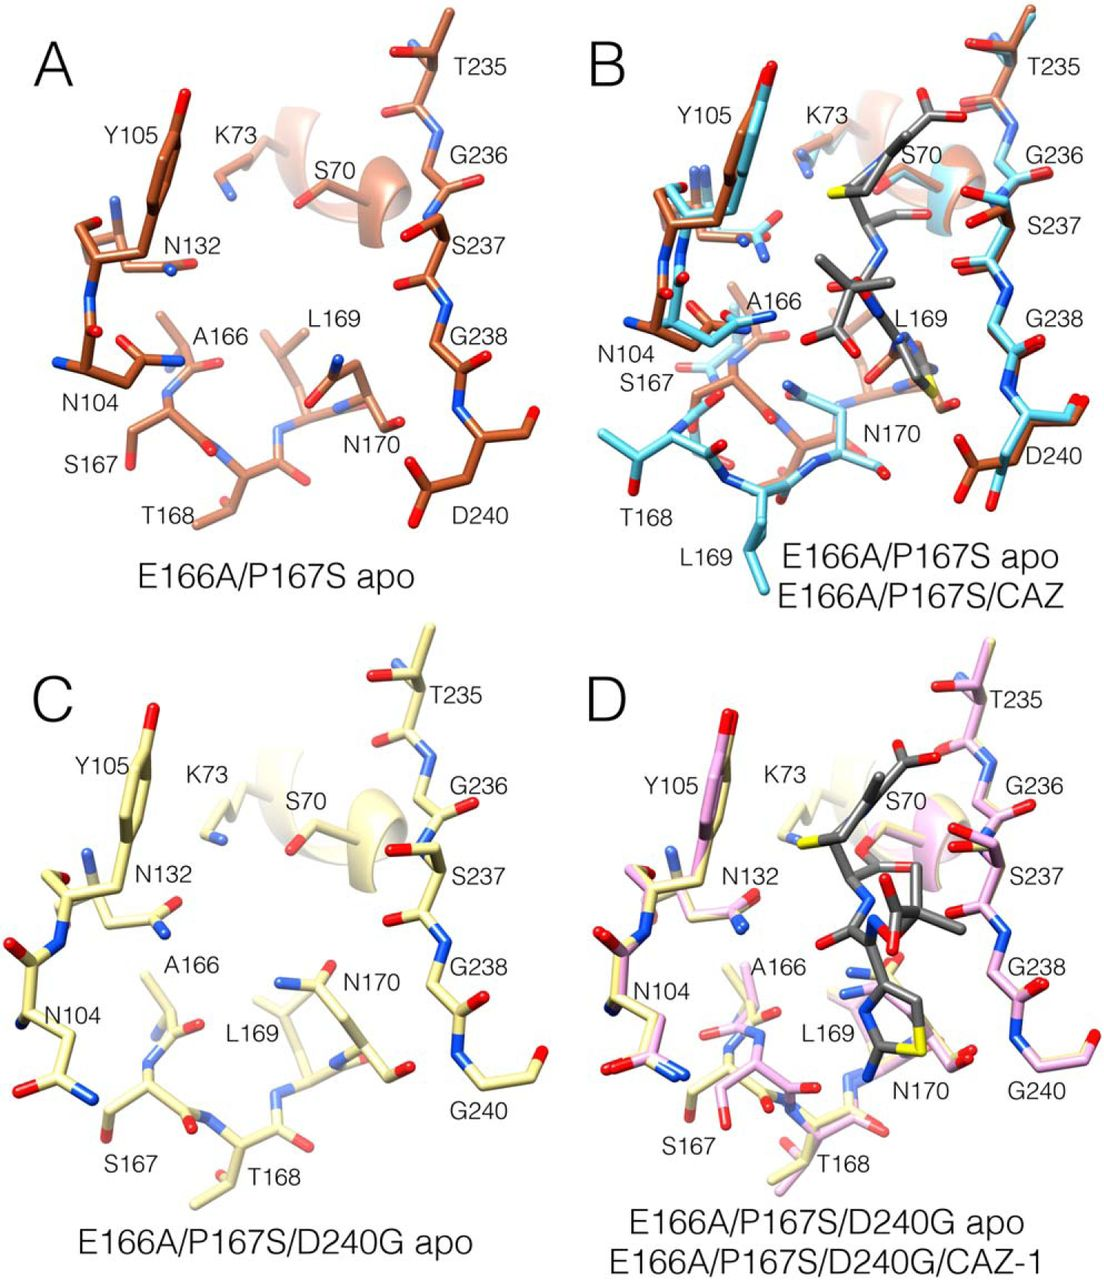
\includegraphics[width=5in]{ch2-fig8.jpg}
            \caption[Structures of the active-site region of CTX-M-14 mutant $\beta$-lactamase acyl-enzyme complexes with ceftazidime.]
                {Structures of the active-site region of CTX-M-14 mutant $\beta$-lactamase acyl-enzyme complexes with ceftazidime. A, structure of the E166A mutant (tan) with ceftazidime (dark gray) trapped in the acyl-enzyme form (PDB code 5U53). Oxygen is shown in red, and nitrogen is in blue. Hydrogen bonds are indicated by thin black lines. Active-site residues are labeled. B, structure of the E166A/P167S/CAZ acyl-enzyme (light blue) (PDB code 5TW6). C, structure of the E166A/D240G/CAZ acyl-enzyme (light green). D, structure of the E166A/P167S/D240G/CAZ-1 acyl-enzyme (pink). E, structure of the E166A/P167S/D240G/CAZ-2 acyl-enzyme (white). F, structural alignment of the E166A/CAZ (tan) and E166A/D240G/CAZ (green) acyl-enzyme complexes. The ceftazidime from the E166A/CAZ structure is shown in dark gray, and that from E166A/D240G/CAZ is shown in white. The $\Omega$-loop region remains folded in the closed form and the ceftazidime occupies a similar position with the aminothiazole ring surface exposed in these structures.}
            \label{fig:ch2-fig8}
        \end{figure}

        The second E166A/P167S/D240G/CAZ structure is superimposable with that of the E166A/P167S/CAZ structure where the peptide bond preceding Ser167 is in the trans configuration, and the $\Omega$-loop is in an unfolded, open conformation to accommodate ceftazidime (Fig. \ref{fig:ch2-fig7}E). Because the P167S enzyme exhibits enhanced ceftazidime hydrolysis, these findings suggest that the conformation of the enzyme in the E166A/P167S/D240G/CAZ-2 structure is competent to hydrolyze ceftazidime.

        The two structures of E166A/P167S/D240G/CAZ with distinct conformations of the enzyme and ceftazidime suggests there are at least two conformational substates of the P167S/D240G enzyme in the presence of ceftazidime. We suggest that the form with the closed $\Omega$-loop and altered 103–106 loop with Asn104 pointed out of the active site does not efficiently hydrolyze ceftazidime, whereas the form with the open $\Omega$-loop is catalytically competent.

    \subsection{Molecular dynamics simulations reveal that conformational heterogeneity of the $\Omega$-loop is greater in the single mutants than in the WT or double mutant.}

        To directly probe the conformational heterogeneity of the $\Omega$-loop and acyl-enzyme complex, we conducted molecular dynamics simulations of the acylated forms of WT, D240G, P167S, and P167S/D240G. In addition to providing atomically detailed models of the distribution of structures that CTX-M adopts, the fact that no chemical reactions occur in these simulations allowed us to include Glu166 and interrogate its interactions with ceftazidime and CTX-M. Simulations of WT were initiated from a crystal structure of the acyl-enzyme complex (PDB code 5U53)\cite{patel_drug-resistant_2017}, and simulations of P167S were initiated based on a previous model of the E166A/P167S/CAZ structure (PDB code 5TW6)\cite{patel_drug-resistant_2017}. Simulations of D240G were initiated from the E166A/D240G/CAZ crystal structure presented in this work. The closed-conformation crystal structure of E166A/P167S/D240G/CAZ-1 was the initial starting structure for simulations of P167S/D240G/CAZ. In all structures, Ala166 was mutated back to a glutamic acid, and a total of 2.5 $\mu$s of simulation was run for each variant.

        The distribution of $\Omega$-loop conformations observed in our simulations suggests a correlation between $\Omega$-loop opening and ceftazidime hydrolysis activity. The WT and P167S/D240G variant with acylated ceftazidime both favor a well-defined closed conformation (Fig. \ref{fig:ch2-fig9}). However, we note that the P167S/D240G variant with acylated ceftazidime sparsely samples open conformations of the $\Omega$-loop, some of which are very similar to the crystallographic structure capturing the open state (Fig. \ref{fig:ch2-fig7}, D and E, and Fig. \ref{fig:ch2-suppfig3}). A previous combination of simulations and experiments have also demonstrated that the WT has a sparsely populated state with an open $\Omega$-loop\cite{Porter:2019hv}. In contrast, the P167S and D240G substitutions dramatically increase the probability of a diversity of open conformations. The conformational heterogeneity of P167S is consistent with the open structure and elevated B-factors observed in the E166A/P167S/CAZ crystal structure (Figs. \ref{fig:ch2-fig6} and \ref{fig:ch2-fig7}B). Although D240G also displays substantial conformational heterogeneity, it has a deeper minima for the closed state than P167S, potentially explaining why only the closed state of D240G has been observed crystallographically so far (Fig. \ref{fig:ch2-fig7}C).

        \begin{figure}[!htb] %Positioning code for figure
            \centering
            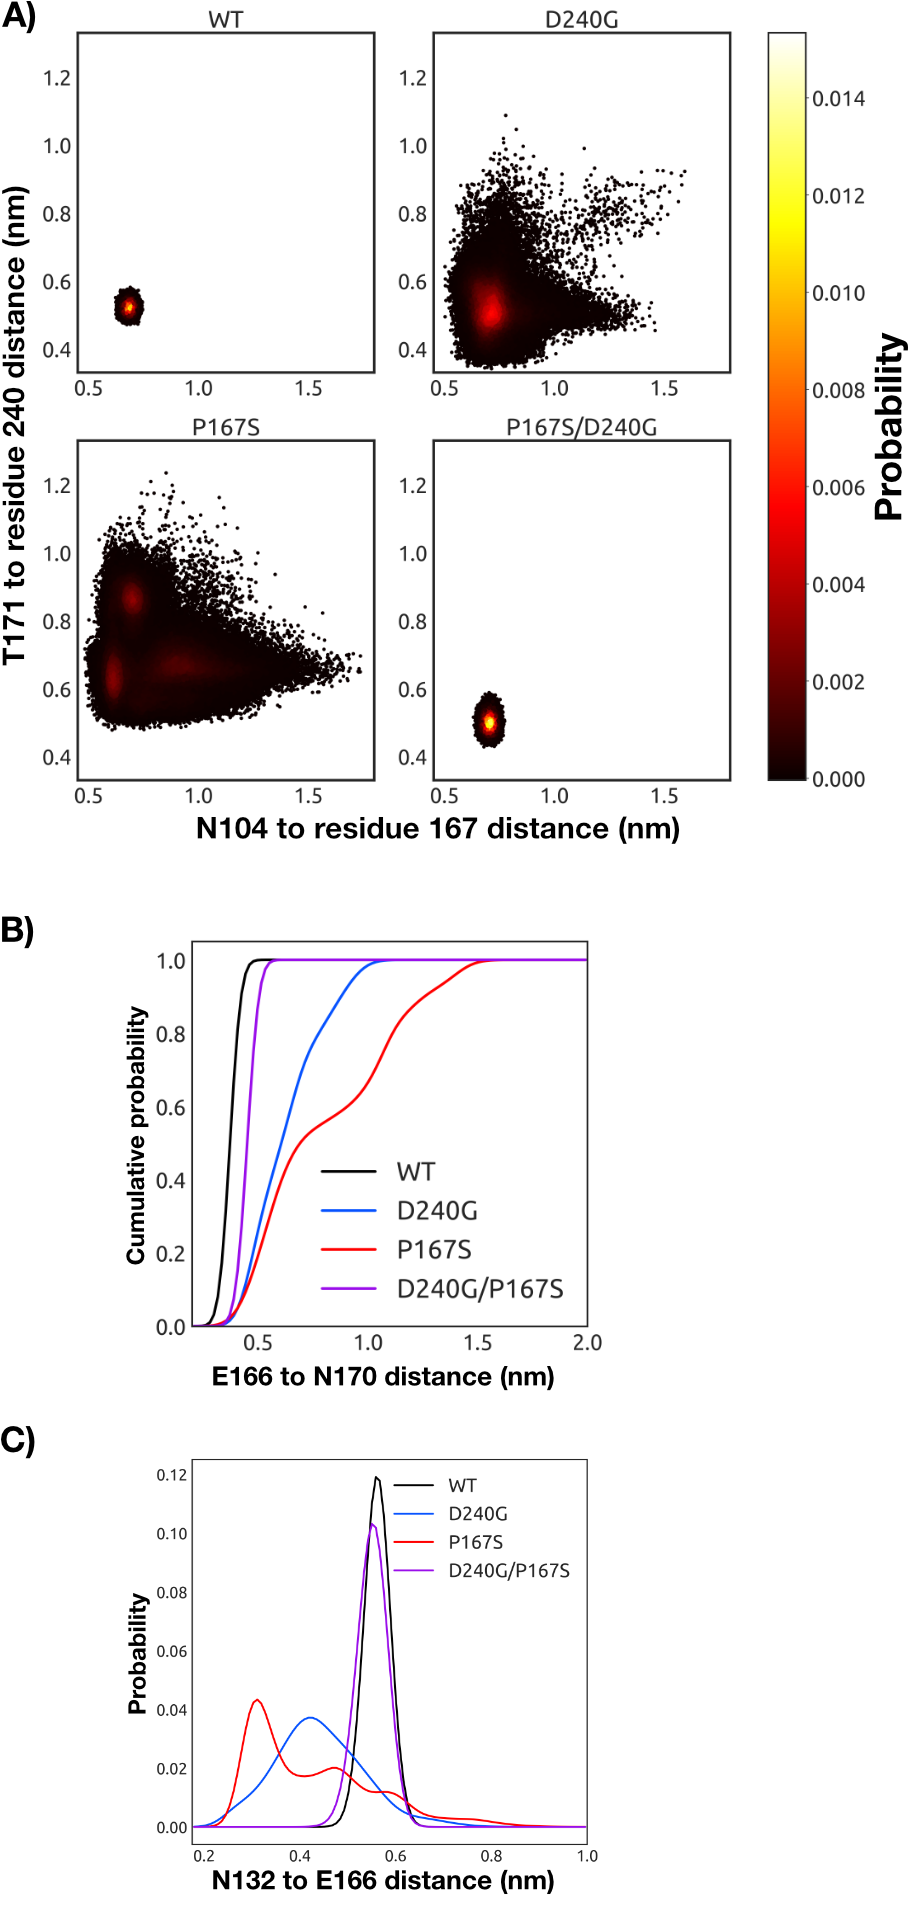
\includegraphics[width=3.2in]{ch2-fig9.png}
            \caption[The conformational heterogeneity of the $\Omega$-loop is greater in the single mutants than in the WT or double mutant.]
                {The conformational heterogeneity of the $\Omega$-loop is greater in the single mutants than in the WT or double mutant. A, joint distributions of two C$\alpha$–C$\alpha$ distances that capture the conformational heterogeneity of the $\Omega$-Loop: (i) Asn104 to position 167 on one side of the $\Omega$-loop and (ii) Thr171 to position 240 on the other side. Distributions are shown for WT (top left panel), D240G (top right panel), P167S (bottom left panel), and P167S/D240G (bottom right panel). Each point represents a snapshot from the molecular dynamics simulations colored according to its probability based on a 2D histogram. B, cumulative distribution of distances between the C$\gamma$ atom of Glu166 and the N$\delta$ atom of Asn170 for WT (black), D240G (blue), P167S (red), and P167S/D240G (purple), capturing the loss of interaction between Glu166 and Asn170 in the open state. C, distribution of distances between the sidechain N$\delta$ atom of Asn132 and the C$\gamma$ of Glu166 for WT (black), D240G (blue), P167S (red), and P167S/D240G (purple), capturing the newly formed interaction between Glu166 and Asn132 in the open state.}
            \label{fig:ch2-fig9}
        \end{figure}

        These simulations suggest that the closed conformation inhibits catalysis by favoring a conformation of Glu166 that is incompatible with a deacylation reaction, whereas the open conformation of the $\Omega$-loop allows Glu166 to adopt a wider range of conformations, at least some of which are compatible with the requirements for deacylation. Previous work has established that Glu166 coordinates a water that plays a role in the deacylation reaction\cite{chen_acylation_2007} and that mutation of Glu166 traps the acyl intermediate by inhibiting deacylation\cite{strynadka_molecular_1992}. Examining closed structures preferentially adopted by WT and P167S/D240G reveals that the carboxyl group of Glu166 tends to hydrogen bond with Asn170, trapping Glu166 under the $\Omega$-loop and preventing it from coordinating the water required for deacylation (Figs. \ref{fig:ch2-fig9}, B and C, and \ref{fig:ch2-fig10}). In the open conformations preferentially sampled by the D240G and P167S variants, the hydrogen bond between Asn170 and Glu166 is disrupted. This open conformation is stabilized by a rearrangement of the hydrogen-bonding network in the active site where Asn132 hydrogen bonds with Glu166 (Figs. \ref{fig:ch2-fig9}C and \ref{fig:ch2-fig10}).

        \begin{figure}[!htb] %Positioning code for figure
            \centering
            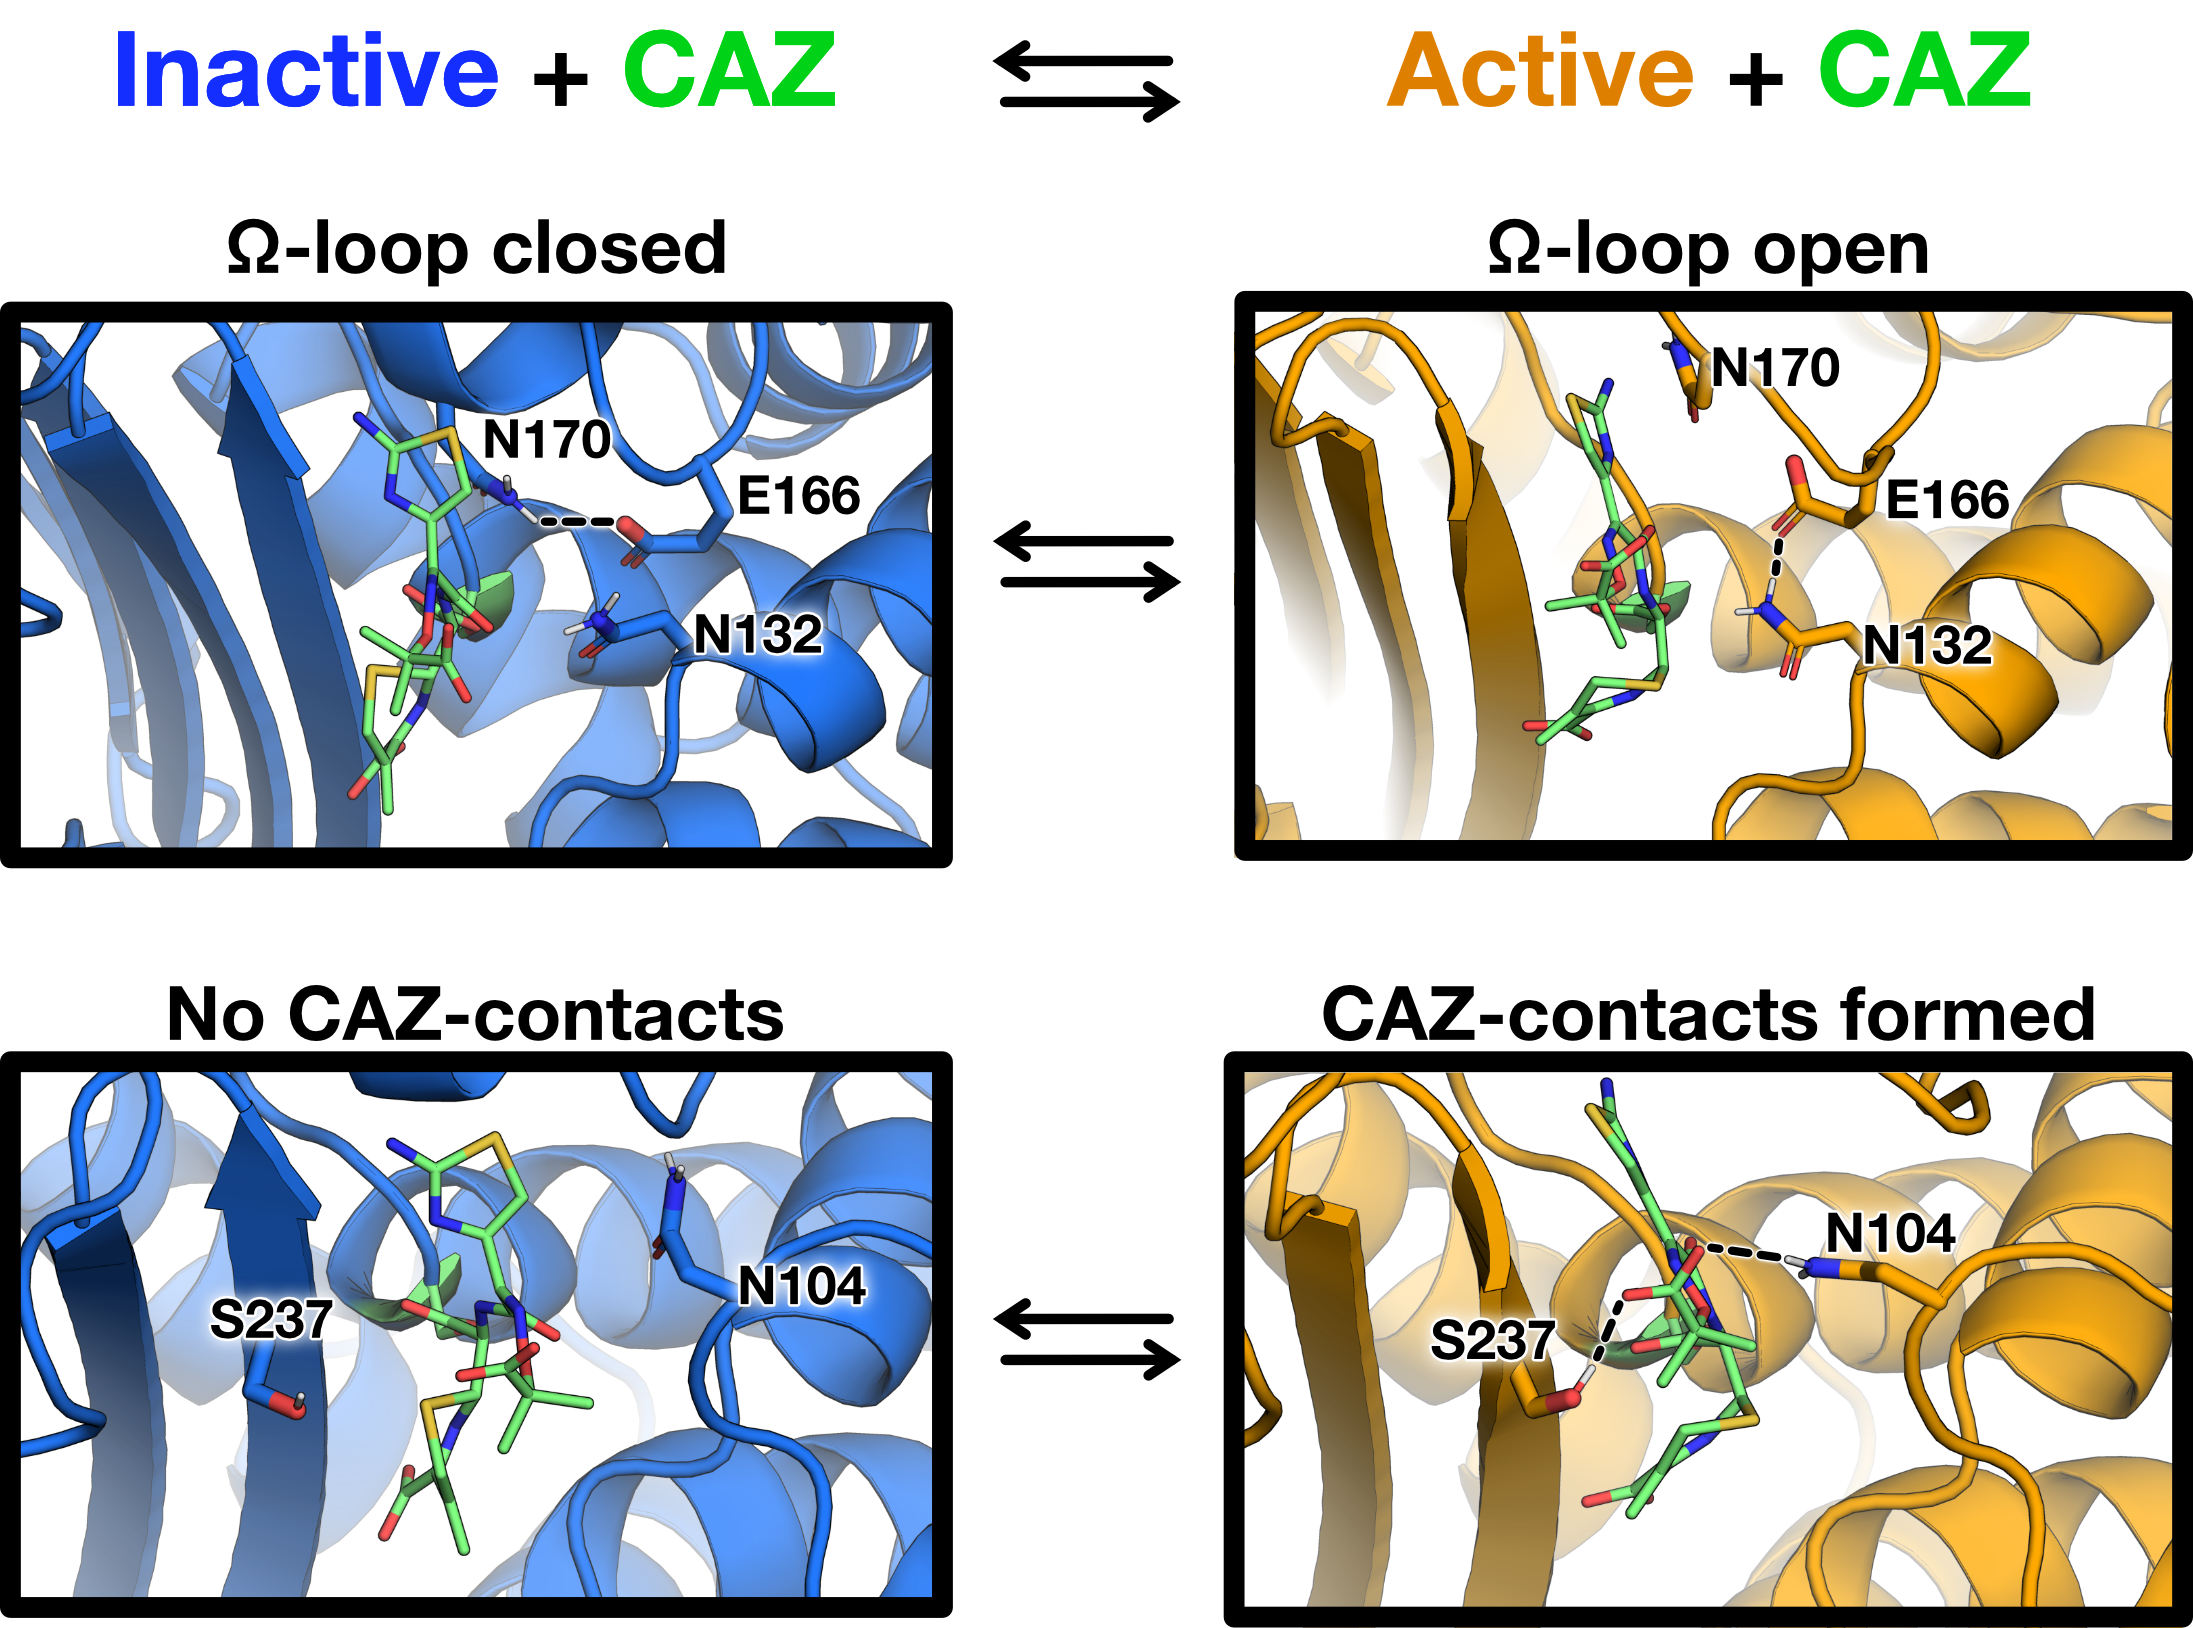
\includegraphics[width=5in]{ch2-fig10.png}
            \caption[Conformational changes between inactive and active forms of the acyl-enzyme.]
                {Conformational changes between inactive and active forms of the acyl-enzyme. Representative structures of the CTX-M acyl-enzyme complex with ceftazidime (labeled CAZ, green) highlighting inactive (blue, left panels) and active (orange, right panels) conformations. Conformations of the $\Omega$-loop (top panels) and residues contacting ceftazidime (bottom panels) are shown, with relevant residues labeled. Key hydrogen bond interactions are depicted in dashed lines (black).}
            \label{fig:ch2-fig10}
        \end{figure}

        The opening and closing of the $\Omega$-loop is also associated with a rearrangement of ceftazidime in the acyl-enzyme complex (Fig. \ref{fig:ch2-fig10} and Fig. \ref{fig:ch2-suppfig1}). One major feature observed in both crystal structures and simulations is that the aminothiazole ring of ceftazidime is buried under the $\Omega$-loop when it is open (Figs. \ref{fig:ch2-fig7}, B and E, and \ref{fig:ch2-fig10}). Consistent with the crystal structures of the single-mutant variants, this rearrangement of ceftazidime in the acyl-enzyme complex is facilitated by new interactions with Asn104 and the $\beta$3 loop. In the D240G and P167S constructs, Ser237 and Asn104 form interactions with ceftazidime (Fig. \ref{fig:ch2-fig10} and Figs. \ref{fig:ch2-suppfig1} and \ref{fig:ch2-suppfig2}). We also note an additional interaction between the imino group of ceftazidime and Ser237 that is present in the more open, active variants but not the more closed, inactive variants (Fig. \ref{fig:ch2-suppfig2}). These interactions with ceftazidime are rare in the WT and P167S/D240G simulations (Figs. \ref{fig:ch2-suppfig1} and \ref{fig:ch2-suppfig2}). Furthermore, Asn104 appears to point outward toward the solvent in the closed configuration (Fig. \ref{fig:ch2-fig10}), similar to what is seen in the crystal structure of the closed configuration of the P167S/D240G/CAZ variant (Fig. \ref{fig:ch2-fig7}D).

        Overall, our simulations suggest that the CTX-M acyl-enzyme complex is in equilibrium between inactive and active conformations and that the P167S and D240G variants have a higher probability of adopting active conformations (Fig. \ref{fig:ch2-fig10}). In the inactive conformation the $\Omega$-loop is closed, burying the Asn170–Glu166 hydrogen bond under the aminothiazole ring (Fig. \ref{fig:ch2-fig10}). Opening of the $\Omega$-loop and rearrangement of ceftazidime via burial of the aminothiazole ring and coordination between the imino group and Asn104 and the $\beta$3 loop likely transitions CTX-M into a catalytically competent state. These rearrangements of the $\Omega$-loop and ceftazidime allow Glu166 to coordinate a water molecule that can access the ester bond of the ceftazidime–acyl-enzyme complex, facilitating the deacylation reaction. Taken together, the crystallography and molecular dynamics results indicate that the P167S and D240G substitutions promote an open conformation of the $\Omega$-loop that creates access for ceftazidime and allows Glu166 to sample conformations consistent with deacylation, whereas the WT and P167S/D240G mutant exhibit a closed $\Omega$-loop conformation that constrains access for ceftazidime and prevents Glu166 from efficiently coordinating water for deacylation.

    \section{Discussion}

        The CTX-M $\beta$-lactamases emerged in the late 1980s and are characterized by their ability to efficiently hydrolyze cephalosporins, particularly the oxyimino-cephalosporin cefotaxime\cite{bonnet_growing_2004,dandrea_ctx-m-type_2013}. For example, the catalytic efficiency for cefotaxime hydrolysis by CTX-M enzymes is 1500-fold higher than that exhibited by the common TEM-1 $\beta$-lactamase\cite{palzkill_structural_2018}. Nevertheless, the related oxyimino-cephalosporin ceftazidime is poorly hydrolyzed by CTX-M enzymes with k$_{cat}$/K$_{m}$ values 1000-fold lower than those observed for cefotaxime\cite{palzkill_structural_2018}. Natural variants of the TEM-1 enzyme have evolved through mutations that provide increased rates of ceftazidime catalysis. Similarly, the P167S and D240G substitutions have been found in multiple variants of CTX-M enzymes that exhibit increased ceftazidime hydrolysis\cite{dandrea_ctx-m-type_2013,bonnet_effect_2003,kimura_role_2004,canton_ctx-m_2012,cartelle_high-level_2004}. Each of these substitutions results in a 10-fold increased k$_{cat}$/K$_{m}$ value for ceftazidime hydrolysis\cite{chen_atomic_2005,patel_characterization_2015}. However, variants containing both substitutions have not been observed, despite the prediction that such variants would exhibit increased hydrolysis. Here we have shown that the failure of the double mutant to emerge in natural isolates is due to epistasis resulting from decreased stability and lower bacterial expression levels of the P167S/D240G enzyme, as well as antagonism between the substitutions with respect to catalysis.

        The combination of amino acid substitutions that each increase catalytic activity can display simple additivity or cooperativity when introduced together into an enzyme\cite{wells_additivity_1990}. For additive interactions, the fold change of the double mutant is expected to be the product of the fold changes of the single mutants. Such additive combinations indicate that the substitutions have independent effects on catalysis\cite{wells_additivity_1990}. However, not all substitutions act additively. The CTX-M P167S and D240G substitutions are antagonizing in the double mutant (Table \ref{tab:ch2-tab2}). This negative cooperativity suggests that the substitutions interact, either directly or indirectly, and that the interaction has a negative effect on ceftazidime catalysis\cite{wells_additivity_1990}. In the case of the P167S and D240G substitutions, the interaction is not via direct contact, because the $\alpha$-carbons are located 10.7 \AA{} apart.

        X-ray crystallography and molecular dynamics simulations of the P167S, D240G, and P167S/D240G mutants provide a rationale for the increased ceftazidime hydrolysis by the single mutants and the negative cooperativity observed for the double mutant. The acyl-enzyme complex of the E166A/P167S/CAZ X-ray structure shows a trans configuration peptide bond preceding residue 167 and an unfolded $\Omega$-loop in an open conformation with the aminothiazole ring of the antibiotic in a buried position. This interaction increases van der Waals contacts and hydrogen bonds between the enzyme and ceftazidime and is consistent with enhanced catalytic efficiency toward ceftazidime. In contrast, the E166A/D240G/CAZ structure revealed a closed conformation. Two structures were obtained for the E166A/P167S/D240G ceftazidime acyl-enzyme, one of which is superimposable with the open $\Omega$-loop structure of E166A/P167S/CAZ and, based on this similarity, is proposed to hydrolyze ceftazidime. The second structure, however, displays a closed $\Omega$-loop and an altered conformation of the 103–106 loop such that the critical Asn104 residue is turned out of the active site and does not interact with ceftazidime, suggesting reduced ceftazidime catalysis.

        Although the E166A/P167S/CAZ and E166A/D240G/CAZ structures suggest that the substitutions act by different mechanisms, 2.5-$\mu$s molecular dynamics simulations of each variant indicate that both the P167S and D240G substitutions promote an open conformation of the $\Omega$-loop to accommodate ceftazidime and that the WT and P167S/D240G enzymes exhibit reduced ceftazidime hydrolysis because open conformations of the $\Omega$-loop are less probable.

        The TEM-1 $\beta$-lactamase is $\sim$35\% identical in amino acid sequence to CTX-M enzymes and efficiently hydrolyzes penicillins and many cephalosporins, but oxyimino-cephalosporins are poor substrates\cite{palzkill_structural_2018}. Nevertheless, natural variants of TEM-1 have evolved that exhibit increased catalytic efficiency for cefotaxime and ceftazidime hydrolysis\cite{petrosino_-lactamases:_1998,salverda_natural_2010}. These variants, termed extended-spectrum $\beta$-lactamases (ESBLs), contain 1–5 amino acid substitutions, and multiply substituted enzymes are common. Many of the substitutions found in these variants act additively when combined\cite{palzkill_structural_2018}. Some combinations of mutations, however, are not additive. A well-studied example is the combination of the R164S and G238S substitutions. The Gly238 residue is on the $\beta$3 strand (analogous to Gly238 in CTX-M-14), and Arg164 is at the base of the $\Omega$-loop. Each of these substitutions results in increased enzyme activity toward cefotaxime and ceftazidime, yet the double mutant has reduced activity\cite{dellus-gur_negative_2015,giakkoupi_detrimental_2000}. Dellus-Gur et al. \cite{dellus-gur_negative_2015} determined the structure of the TEM-1 G238S and R164S enzymes. The G238S-containing enzyme exhibited two dominant conformations of the G238 loop, whereas the R164S substitution induced an ensemble of conformations of the $\Omega$-loop. The structure of the R164S/G238S double mutant, however, exhibited a wider ensemble of conformations of the $\Omega$-loop than the single mutants\cite{dellus-gur_negative_2015}. Based on these results, it was hypothesized that the entropic cost of the substrate selecting suitable conformations among many alternatives results in the low activity for cefotaxime hydrolysis by the double mutant, accounting for the negative epistasis observed for the combination\cite{dellus-gur_negative_2015}.

        In the case of the negative epistasis observed with the P167S and D240G combination in CTX-M $\beta$-lactamase, multiple conformations of the enzyme also appear to play a role. Based on our molecular dynamics simulation results, the P167S and D240G substitutions are analogous to the R164S substitution in TEM-1, where the substitutions induce an ensemble of conformations, some of which are predicted to be capable of hydrolyzing ceftazidime. The CTX-M P167S and D240G substitutions antagonize each other in the double mutant, similar to the TEM-1 R164S and G238S substitutions. The mechanism of antagonism, however, is different, with the CTX-M P167S/D240G double mutant showing a reduced probability of sampling multiple conformations of the $\Omega$-loop, whereas the TEM-1 R164S/G238S double mutant $\Omega$-loop samples an excess of conformations\cite{dellus-gur_negative_2015}. Nevertheless, both cases demonstrate the importance of conformational heterogeneity of active-site loops in controlling catalytic activity and evolutionary trajectories.

        Several studies have provided evidence that the conformation of the $\Omega$-loop is an important determinant of substrate specificity of class A $\beta$-lactamases, particularly with regard to the hydrolysis of oxyimino-cephalosporins. As described above, the TEM ESBL mutation R164S is thought to broaden the specificity of the enzyme by increasing the conformational heterogeneity of the $\Omega$-loop\cite{dellus-gur_negative_2015}. In addition, the structure of an apo enzyme form of a triple mutant of the TEM enzyme containing the substitutions W165Y/E166Y/P167G that hydrolyzes ceftazidime shows the $\Omega$-loop in an unfolded, open conformation similar to that observed for the CTX-M E166A/P167S/CAZ and E166A/P167S/D240G/CAZ-2 structures\cite{stojanoski_triple_2015}. Further, computational studies predict that TEM ESBL substitutions that broaden the specificity of the enzyme to include cefotaxime stabilize conformations of the $\Omega$-loop that facilitate substrate binding\cite{Hart:2016kb}.

        The results also suggest an important role for the active-site 103–106 loop in cefotaxime and ceftazidime hydrolysis. We recently showed that an N106S mutation in the 103–106 loop that is found in CTX-M enzymes from clinical isolates lowers cefotaxime and ceftazidime hydrolysis because of a change in conformation of the loop\cite{patel_synergistic_2018}. Asn106 is at the base of the loop and not in the active site. However, the N106S substitution changes the hydrogen-bonding network connectivity in the loop such that the side chain of Asn104 rotates out of the active site, thereby eliminating a hydrogen bond with substrate. Further experiments showed that an N104A mutant exhibits 10-fold reduced catalytic efficiency for oxyimino cephalosporin hydrolysis, suggesting that the hydrogen bond is important for catalysis. Thus, the conformation of the 103–106 loop is a determinant of substrate specificity\cite{patel_synergistic_2018}. In this study, it was found that the P167S/D240G enzyme, which exhibits reduced ceftazidime hydrolysis, has increased B-factors for the 103–106 loop, suggesting disorder in Asn104 that is consistent with reduced activity. In addition, in the structure of the E166A/P167S/D240 apo enzyme the B-factors of the 103–106 loop are increased, and in one of the structures of E166A/P167S/D240G in complex with ceftazidime, the side chain of Asn104 is rotated out of the active site, again consistent with decreased ceftazidime hydrolysis. Thus, although the P167S and D240G substitutions are not in the 103–106 loop, the antagonism between the substitutions is at least partially reflected in changes in the conformation of the loop.

        Thermal stability studies of the WT, P167S, D240G, and P167S/D240G enzymes show that the single mutants are less stable than WT, whereas the double mutant is less stable than either single mutant. There is some correlation between stability and protein expression levels in that the P167S/D240G mutant is the least stable and is also expressed at the lowest levels among the mutants. However, also note the P167S mutant is less stable than D240G but is expressed at higher levels, suggesting there are exceptions to the stability/protein expression level correlation. Some recent studies have shown that lower enzyme stability correlates with increased flexibility and increased cephalosporin hydrolysis in $\beta$-lactamases\cite{frohlich_oxa-48-mediated_2019,barnes_deciphering_2018}. Here, we do not observe a correlation between stability and flexibility in that the P167S and D240G mutants readily sample multiple conformations and yet are more stable than P167S/D240G, which samples fewer conformations. Further, we do not observe a correlation between stability and catalytic activity toward ceftazidime because P167S/D240G has low stability but also low activity.

        Taken together, the results presented here suggest that active-site loops play an important role in the substrate specificity and evolutionary capacity of $\beta$-lactamases. Class A $\beta$-lactamases such as TEM and CTX-M can evolve altered substrate specificity by mutations that change the conformation of active-site loops. An active site with flexible loops loosely associated with a highly ordered, stable scaffold structure has been described as fold polarity, and there is evidence that such an organization facilitates the evolution of new functions because of a tolerance to changes in the loops without drastically destabilizing the enzyme\cite{dellus-gur_what_2013}. Such an organization is clearly advantageous for antibiotic resistance enzymes such as CTX-M $\beta$-lactamases that are under selective pressure for altered substrate specificity.

    \section{Methods}
    \subsection{Bacterial strains and plasmids.}
        The CTX-M-14-pTP123 plasmid was used for site-directed mutagenesis, MIC determinations, and immunoblotting. This plasmid was constructed by inserting the blaCTX-M-14 gene into the previously described pTP123 plasmid. CTX-M-14-pTP123 has a chloramphenicol (CMP) resistance marker and $\beta-$-lactamase expression is controlled by the isopropyl$-\beta-$-D-galactopyranoside (IPTG)–inducible P$_{trc}$ promoter\cite{petrosino_contributions_1999}. Under conditions without IPTG, protein expression is maintained at a basal level; these were the conditions under which MIC determination and immunoblotting were performed. The E. coli strain XL1-Blue (recA1 endA1 gyrA96 thi-1 hsdR17 supE44 relA1 lac [F9 proAB lacI$^q$ZM15 Tn10 (Tet$^r$)]) (Stratagene, Inc., La Jolla, CA) was used as the host for the construction of the P167S/D240G CTX-M-14 mutant via site-directed mutagenesis, as well as MIC determination. The E. coli strain RB791 (W3110 lacIqL8) was used as the host for the determination of protein expression levels of WT CTX-M-14 $\beta$-lactamase and its mutants\cite{amann_vectors_1983}. For protein purification, WT CTX-M-14 and the mutants were expressed in the pET28a plasmid using the protocol outlined by Patel et al.\cite{patel_characterization_2015}. CTX-M-14 and mutants in the pET28a plasmid were expressed in BL21(DE3) [fhuA2 (lon) ompT gal ($\lambda$ DE3) (dcm) $\Delta$hsdS $\lambda$ DE3 = $\lambda$sBamHIo $\Delta$EcoRI-B int::(lacI::PlacUV5::T7 gene1) i21 $\Delta$nin5]\cite{studier_use_1986}.

    \subsection{Site-directed mutagenesis.}
        The CTX-M-14 P167S/D240G mutant was constructed using the D240G mutant in pTP123 as template for QuikChange mutagenesis using 1 unit of Phusion DNA polymerase (New England Biolabs, Ipswich, MA) and 0.4 $\mu$M P167S primer (5'-CTGGATCGCACTGAAAGCACGCTGAATACCGCC-3')\cite{patel_characterization_2015}. Primers were obtained from Integrated DNA Technologies (Coralville, IA). Thermocycler products were digested with DpnI (New England Biolabs) and transformed into electrocompetent E. coli XL1-Blue cells and selected on LB agar supplemented with 12.5 $\mu$g/ml chloramphenicol. The DNA sequence of the resulting mutant was confirmed by DNA sequencing (Genewiz, Plainfield, NJ). The E166A/P167S/D240G mutant was constructed by QuikChange mutagenesis with a primer encoding the E166A/P167S mutations (5'-GATCGCACTGCTCCTACGCTGAAT-3') using CTX-M-14 P167S/D240G pTP123 as template and confirmed using DNA sequencing.

    \subsection{Minimum inhibitory concentration determinations.}
        MICs for cephalothin were determined by Etest strip (BioMérieux, Marcy-l'Étoile, France). This was performed by growing a single colony of E. coli XL1-Blue harboring the pTP123 plasmid with either WT, mutant CTX-M-14, or empty vector overnight in LB supplemented with 12.5 $\mu$g/ml CMP in a shaking incubator at 37 °C. The overnight culture was diluted 10$^{2}$ and spread onto LB agar containing CMP, an Etest strip was placed on the agar, and the MIC was determined based on the zone of inhibition.

        MIC determinations for cefotaxime were performed by broth dilution. Again, a single colony of E. coli XL1-Blue harboring pTP123 with WT or mutant CTX-M-14 or empty vector was grown overnight in LB with CMP in a shaking incubator at 37 °C. The cultures were diluted 10$^{4}$, and 100 $\mu$l of culture was used to inoculate 2 ml of LB supplemented with increasing concentrations of cefotaxime in 14-ml test tubes. Concentrations of cefotaxime (in $\mu$g/ml) used for WT and D240G were 0, 1, 1.5, 2, and 3. The concentrations used for the P167S and P167S/D240G mutants were 0, 0.1875, 0.25, 0.375, and 0.5, and for pTP123 empty vector control, the concentrations were 0, 0.03, 0.045, and 0.06. The cultures were incubated with shaking for 18 h at 37 °C. The concentration at which no visible growth was observed was reported as the MIC.

        MIC determinations for ceftazidime were performed by broth dilution, with a single colony of E. coli XL1-Blue harboring pTP123 with WT or mutant CTX-M-14 or empty vector being grown overnight in LB with CMP, as above. Saturated cultures were diluted 104, and 25 $\mu$l was used to inoculate 500 $\mu$l of LB supplemented with increasing concentrations of ceftazidime in a deep-well 96-well plate. Concentrations of ceftazidime (in $\mu$g/ml) used for WT, D240G, P167S/D240G, and pTP123 empty vector were 0, 0.12, 0.19, 0.25, 0.38, 0.5, 0.75, 1, 1.5, 2, 3, and 4; for P167S, the concentrations were 0, 0.38, 0.5, 0.75, 1, 1.5, 2, 4, 6, 8, and 12. The 96-well plate was covered with a sterile, breathable seal (Excel Scientific, Victorville, CA) and incubated shaking at 37 °C for 18 h. The concentration at which no growth was observed (A$_{600} <$ 0.1) was recorded as the MIC.

    \subsection{Immunoblotting.}
        To determine the effects of the P167S/D240G mutation on steady-state protein expression, single colonies of E. coli RB791 harboring pTP123 or the recombinant pTP123 encoding WT or mutant CTX-M-14 $\beta$-lactamase were incubated overnight with shaking in 2× YT medium supplemented with 12.5 $\mu$g/ml CMP at 37 °C. A total of 10 ml of 2× YT medium with CMP was inoculated with 100 $\mu$l of overnight culture and incubated at 37 °C while shaking until the A600 reached between 0.9. The cells were pelleted, and the periplasmic proteins were extracted by osmotic shock as described previously\cite{patel_synergistic_2018}. The proteins were fractionated by SDS-PAGE and transferred onto a nitrocellulose membrane (GE Healthcare). The membrane was probed with a rabbit serum raised against CTX-M-14 protein and a rabbit serum raised against maltose-binding protein (MBP) (a gift from Dr. Anna Konovalova, University of Texas Health Science Center at Houston), which functions as a loading control. Then the membrane was probed with a donkey anti-rabbit secondary antibody conjugated with horseradish peroxidase (GE Healthcare). After development of the immunoblot with the SuperSignal West Pico chemiluminescent substrate (Thermo Fisher Scientific), the hybridization signals of CTX-M-14 $\beta$-lactamase and MBP were quantified by densitometry using ImageJ software (National Institutes of Health). The signal for WT and mutant CTX-M-14 $\beta$-lactamase was normalized to that for MBP.

    \subsection{Protein purification.}
        WT CTX-M-14 $\beta$-lactamase and the P167S/D240G mutant were expressed from a pET28a vector in E. coli BL21(DE3) cells. Proteins expressed in this plasmid have an N-terminal His tag with a TEV protease cleavage site. E. coli BL21(DE3) cells harboring the CTX-M-14 plasmid were used to inoculate LB supplemented with 25 $\mu$g/ml kanamycin and incubated at 37 °C in a shaking incubator until the A600 reached $\sim$0.9, at which time IPTG was added to yield a final concentration of 0.2 mM to induce protein expression. The culture was then grown for 20 h at 23 °C in a shaking incubator. The culture was centrifuged at 8000 rpm at 4 °C, and the pellet was stored overnight at -80 °C. The pellet was then thawed on ice and resuspended in 30 ml of lysis buffer (20 mM HEPES, pH 7.4, 300 mM NaCl, 20 mM imidazole). The cells were lysed using a French Press at 1250 p.s.i. and a probe sonicator, followed by centrifugation for 50 min at 10,000 rpm and filtration of the supernatant with a 0.45-$\mu$m filter (EMD Millipore, Billerica, MA). Filtered lysate was then bound to a HisTrap FF column (GE Healthcare) equilibrated with the lysis buffer. The CTX-M-14 enzyme was eluted using 20–500 mM imidazole gradient in the lysis buffer. Pure fractions containing His-CTX-M-14 protein were pooled, concentrated, and buffer-exchanged to the lysis buffer using 10-kDa molecular mass cutoff centrifugal filters (EMD Millipore). 0.25 mg of TEV protease was added to the His-tagged enzyme and incubated overnight at 4 °C. TEV protease and uncleaved His-CTX-M-14 protein were removed by incubation with nickel–Sepharose Hi-Performance beads (GE Healthcare). CTX-M-14 proteins were further purified by gel-filtration chromatography with Superdex 75 Increase column using (20 mM HEPES, pH 7.4, 150 mM NaCl) as running buffer. The fractions corresponding to monomer of CTX-M-14 WT or P167S/D240G mutant protein were pooled and concentrated with 10-kDa molecular mass cutoff centrifugal filters. The purity of purified proteins was $>$95\% determined by SDS-PAGE. Their concentrations were determined by measuring the absorbance at 280 nm with DU800 spectrophotometer (BecK$_{m}$an Coulter) and using an extinction coefficient of 23, 950 M$^{-1}$ cm$^{-1}$.

    \subsection{Determination of thermal stabilities.}
        Thermal stabilities of the WT and mutant enzymes were determined as previously described\cite{patel_characterization_2015}. In short, the fraction of folded protein was measured with a spectropolarimeter at 222 nm, while the temperature was increased from 30 to 70 °C at a rate of 0.01 °C/s. The melting temperature (T$_{m}$), the temperature midpoint of protein unfolding, was determined by fitting the data to a single Boltzmann two-state model using GraphPad Prism 6 (San Diego, CA)\cite{brown_multiple_2010}.

    \subsection{Steady-state enzyme kinetic parameters.}
        Michaelis–Menten steady-state kinetic parameters were measured as previously described\cite{patel_characterization_2015,marciano_genetic_2008}. The kinetic parameters for CTX-M-14 P167S and D240G are from Patel et al.\cite{patel_characterization_2015}. Antibiotic hydrolysis was measured at 30 °C in 50 mM phosphate buffer (pH 7.0) containing 1 $\mu$g/ml BSA. BSA was added to stabilize $\beta$-lactamase when it is diluted to low concentration for kinetic assays. Cephalothin, cefotaxime, and ceftazidime hydrolysis were measured at 262, 264, and 260 nm, respectively\cite{patel_characterization_2015}. K$_{m}$ and k$_{cat}$ were determined by fitting the initial velocities of increasing substrate concentrations to the Michaelis–Menten equation using GraphPad Prism 6. For ceftazidime, which has a K$_{m}$ $>$ 500 $\mu$M, k$_{cat}$/K$_{m}$ was estimated using the equation, v = k$_{cat}$/K$_{m}$[E][S], where [S] $\ll$ K$_{m}$. All measurements were performed at least in duplicate. k$_{cat}$ and K$_{m}$ values from each run were averaged, and the standard deviations reported are the sums of the percent standard deviations of k$_{cat}$ and K$_{m}$\cite{patel_characterization_2015}.

    \subsection{Protein crystallization and structure determination.}
        Crystallization conditions were screened based on previously solved crystal structures for CTX-M-14. Purified P167S/D240G enzyme in 50 mM phosphate buffer, pH 7.0, was concentrated to 40 mg/ml, and protein was mixed with mother liquor 1:1 in a 200-nl drop and grown by hanging-drop vapor diffusion. Diffraction-quality crystals were obtained in 0.1 M MIB buffer (malonic acid, imidazole, and boric acid buffer), pH 4.0, 25\% (w/v) PEG 1500, and were harvested and cryoprotected in 25\% glycerol: 75\% mother liquor. The crystals were plunged in liquid nitrogen and sent to Beamline 5.0.2 at the Advanced Light Source (Berkeley, CA) for data collection. Because the first data set appeared to show high twinning, a second data set was collected on the same crystal. This data set was processed at 1.5 \AA{} in the space group P41212 using HKL200 and the Phaser program from the CCP4 suite was used for molecular replacement. CTX-M-14 (PDB code 1YLT) was used as a phasing model\cite{chen_atomic_2005}. Refinement was performed using REFMAC5 and phenix.refine, as part of the Phenix program suite\cite{adams_phenix_2010}. The model was built manually using COOT\cite{emsley_features_2010}.

        E166A/P167S/D240G was crystallized by concentrating the protein in 50 mM phosphate buffer, pH 7.0, to 40 mg/ml and mixing with mother liquor 1:1 in a 200-nl drop and grown by hanging-drop vapor diffusion. Crystals from the condition containing 0.1 M PCB buffer, pH 6, 25\% (w/v) PEG 1500 were soaked for 24 h in 25 mM ceftazidime, 20\% glycerol:80\% mother liquor. Structure determination indicated an acyl-enzyme complex with ceftazidime. Crystals grown in the condition containing 0.2 M CaCl, 0.1 M sodium acetate, pH 5, 20\% (w/v) PEG 6000 were also soaked for 24 h in 25 mM ceftazidime, 20\% glycerol:80\% mother liquor but were not in complex with ceftazidime, resulting in the apoenzyme. The data were collected on Beamline ALS 501 and was processed as described above. The E166A/P167S/D240G enzyme was also crystallized by concentrating the protein in 50 mM phosphate buffer, pH 7.0, to 36 mg/ml, mixing with mother liquor 1:1 in a 200-nl drop, and grown by hanging-drop vapor diffusion. Crystals obtained in the condition 0.1 M MMT (1:2:2 ratio of DL-malic acid:MES:Tris base), pH 6.0, 25\% (w/v) PEG 1500 were soaked for 24 h in 25 mM ceftazidime, 25\% glycerol:75\% mother liquor. The data were collected on Beamline ALS 821. Structure determination revealed an acyl-enzyme complex with ceftazidime with the $\Omega$-loop in an open conformation.

        E166A/D240G was crystallized by concentrating the protein in 50 mM phosphate buffer, pH 7.0, to 36 mg/ml and mixing with mother liquor 1:1 in a 200-nl drop and grown by hanging-drop vapor diffusion. Crystals grown in 0.1 M Tris-HCl, pH 8.5, 25\% (w/v) PEG 3000 were soaked for 24 h in 25 mM ceftazidime, 25\% glycerol:75\% mother liquor. The data were collected on Beamline ALS 822. However, structure determination revealed this to be the apo enzyme. Crystals grown in the condition 0.2 M NaCl, 0.1 M Tris, pH 8.0, 20\% (w/v) PEG 6000 were soaked for 24 h in 15 mM ceftazidime, 25\% glycerol:75\% mother liquor, the data were collected on Beamline ALS 822, and structure determination revealed an acyl-enzyme complex with ceftazidime. The data set was processed as described above for the P167S/D240G enzyme. X-ray crystallography statistics are listed in Table \ref{tab:ch2-supptable1}.

    \subsection{Molecular dynamics simulations.}
        As described previously\cite{Hart:2016kb}, simulations were run at 300 K with the GROMACS software package\cite{Hart:2016kb,Berendsen:1995dd,Abraham:2015gj,VanDerSpoel:2005hz} using the Amber03 force field\cite{Duan:2003gt} and TIP3P explicit solvent\cite{Jorgensen:1983fl}. Mutations were introduced in PyMOL\cite{DeLano:2010wf}, and parameters for the acyl group were generated with the generalized amber force field\cite{sousa_da_silva_acpype_2012,wang_development_2004,wang_automatic_2006}. A total of 2.5 $\mu$ s of simulation were run for each variant.




    \section{Author contributions}
    C. A. B., B. V. V. P., G. R. B., and T. P. conceptualization; C. A. B., L.H., Z.S., M.P.P., S.S., J.R.P., and B.S. investigation; C. A. B., L.H., Z.S., M.P.P., S.S., J.R.P., and B.S. methodology; C. A. B. and T. P. writing-original draft; C. A. B., L.H., Z.S., M.P.P., S.S., J.R.P., B.S., B. V. V. P., G. R. B., and T. P. writing-review and editing; L.H., Z.S., S.S., J.R.P., B.S., B. V. V. P., G. R. B., and T. P. formal analysis; Z.S. data curation; S.S. visualization; B. V. V. P., G. R. B., and T. P. supervision; B. V. V. P., G. R. B., and T. P. funding acquisition.


       
    \section{Acknowledgments}
        We thank Hiram Gilbert for discussions and comments on the manuscript. The ALS-ENABLE Beamlines are supported in part by National Institutes of Health, NIGMS Grant P30 GM124169-01. The Advanced Light Source is a Department of Energy Office of Science User Facility under Contract DE-AC02-05CH11231.

        This work was supported by National Institutes of Health Grants R01 AI32956 (to T. P.) and R01 GM12400701 (to G. R. B.) and by Robert Welch Foundation Grant Q1279 (to B. V. V. P.). The authors declare that they have no conflicts of interest with the contents of this article. The content is solely the responsibility of the authors and does not necessarily represent the official views of the National Institutes of Health.

    \section{Additional information.}
        The atomic coordinates and structure factors (codes 6V5E, 6V6G, 6V6P, 6V7T, 6V8V, and 6V83) have been deposited in the Protein Data Bank (http://wwpdb.org/).

        \begin{table}[]
        \centering
        \caption[Abbreviations used in chapter 2]{The abbreviations used are:}
        \label{tab:ch2-abbreviation-table}
        \begin{tabular}{ll}
        \textbf{Abbreviation}  & \textbf{Expanded name}                    \\ \hline
        \textbf{MIC}  & \textit{Minimum inhibitory concentration} \\ \hline
        \textbf{PDB}  & \textit{Protein data bank}                \\ \hline
        \textbf{ESBL} & \textit{Extended spectrum $\beta$-lactamase}    \\ \hline
        \textbf{CMP}  & \textit{chloramphenicol}                  \\ \hline
        \textbf{IPTG} & \textit{isopropyl-$\beta$-D-galactopyranoside}  \\ \hline
        \textbf{MBP}  & \textit{maltose-binding protein}         
        \end{tabular}
        \end{table}


%     \section{Supplemental material}
%         \renewcommand{\thefigure}{\arabic{chapter}.S\arabic{figure}}
%         \setcounter{figure}{0}

%         \begin{table}[]
%         \centering
%         \caption[X-ray crystallography data collection and refinement statistics for CTX-M-14 mutant enzymes.]{X-ray crystallography data collection and refinement statistics for CTX-M-14 mutant enzymes. }
%         \label{tab:ch2-supptable1}
%         \resizebox{\textwidth}{!}{\begin{tabular}{|l|l|l|l|l|l|l|}
%         \hline
%                                       & P167S/D240G & E166A/D240G & E166A/P167S/ & E166A/D240G- & E166A/P167S/ & E166A/P167S/ \\ \hline
%                                       &             &             & D240G        & CTX          & D240G-CTX-1  & D240G-CTX-2  \\ \hline
%         PDB ID                        & 6V5E        & 6V6P        & 6V6G         & 6V7T         & 6V83         & 6V8V         \\ \hline
%         Data collection               &             &             &              &              &              &              \\ \hline
%         Space group                   & P 41 21 2   & P 41 21 2   & P 32 2 1     & P 21         & P 41 21 2    & P 32 2 1     \\ \hline
%         a, b, c ()                & 42.2, 42,2, 261.6 & 41.9, 41.9, 259.2 & 41.4, 41.4, 231.1 & 45.1, 107.3, 47.8 & 42.4, 42.4, 262.7 & 41.3, 41.3, 231.6 \\ \hline
%         $\alpha$, $\beta$, $\gamma$ (°)               & 90, 90, 90        & 90, 90, 90        & 90, 90, 120       & 90, 99.9, 90      & 90, 90, 90        & 90, 90, 120       \\ \hline
%         Resolution Range (\AA{})      & 41.70 - 2.30      & 39.89 - 1.55      & 35.88 - 1.50      & 35.48 - 1.34      & 41.82 - 1.80      & 32.44 - 1.80      \\ \hline
%                                   & (2.38 - 2.30)     & (1.61 - 1.55)     & (1.56 - 1.50)     & (1.39 - 1.34)     & (1.84 - 1.80)     & (1.87 - 1.80)     \\ \hline
%         R-merge (\%)                  & 8.4 (12.1)  & 9.7 (18.7)  & 5.6 (46.5)   & 4.7 (11.8)   & 9.4 (60.6)   & 8.7 (11.8)   \\ \hline
%         I/sigma                       & 17.4 (9.6)  & 16.6 (10.3) & 30.8 (5.1)   & 17.1 (8.5)   & 31.3 (5.4)   & 11.7 (4.8)   \\ \hline
%         Multiplicity                  & 7.0 (6.4)   & 11.8 (14.0) & 8.4 (10.6)   & 3.7 (3.7)    & 16.7 (19.9)  & 4.8 (2.0)    \\ \hline
%         Completeness (\%)             & 88.3        & 85.5        & 98.8         & 99.4         & 100          & 97.9         \\ \hline
%         Wilson B-factor ($\AA{}^2$)          & 29.4        & 10.3        & 12.1         & 9.1          & 18.2         & 14.1         \\ \hline
%                                       &             &             &              &              &              &              \\ \hline
%         Refinement                    &             &             &              &              &              &              \\ \hline
%         Molecules per asymmetric unit & 1           & 1           & 1            & 2            & 1            & 1            \\ \hline
%         No. of unique reflections & 10104 (880)       & 30051 (2829)      & 37869 (3494)      & 99523 (9924)      & 23526 (2299)      & 21924 (1871)      \\ \hline
%         R-work/R-free (\%)        & 18.5 / 25.1       & 16.8 / 19.4       & 18.3 / 21.7       & 14.3 / 16.1       & 17.1 / 20.8       & 14.9 / 18.9       \\ \hline
%         No. of protein residues       & 263         & 263         & 260          & 526          & 261          & 260          \\ \hline
%         Ramachandran                  &             &             &              &              &              &              \\ \hline
%         Favored (\%)                  & 98.5        & 98.1        & 97.7         & 98.1         & 98.5         & 98.1         \\ \hline
%         Outliers (\%)                 & 0           & 0           & 0.39         & 0.38         & 0            & 0.39         \\ \hline
%         Average B-factor ($\AA{}^2$)         & 31          & 14.2        & 21.2         & 14.1         & 23.3         & 16.6         \\ \hline
%         Protein                       & 30.8        & 12.4        & 19.6         & 11.7         & 21.1         & 14.4         \\ \hline
%         Ligand                        & -           & 23.4        & 37.3         & 18.6         & 62.2         & 28.7         \\ \hline
%         Solvent                       & 34.7        & 29.1        & 32.1         & 26.7         & 36.3         & 30.2         \\ \hline
%         RMS deviations                &             &             &              &              &              &              \\ \hline
%         Bond length ($\AA{}$)               & 0.003       & 0.011       & 0.007        & 0.006        & 0.006        & 0.011        \\ \hline
%         Bond angles (°)               & 0.685       & 1.16        & 0.92         & 0.93         & 0.96         & 1.204        \\ \hline
%         \end{tabular}}
%         \textit{*Values in parentheses represent the highest-resolution bin.}
%         \end{table}

%         \begin{figure}[!htb] %Positioning code for figure
%             \centering
%             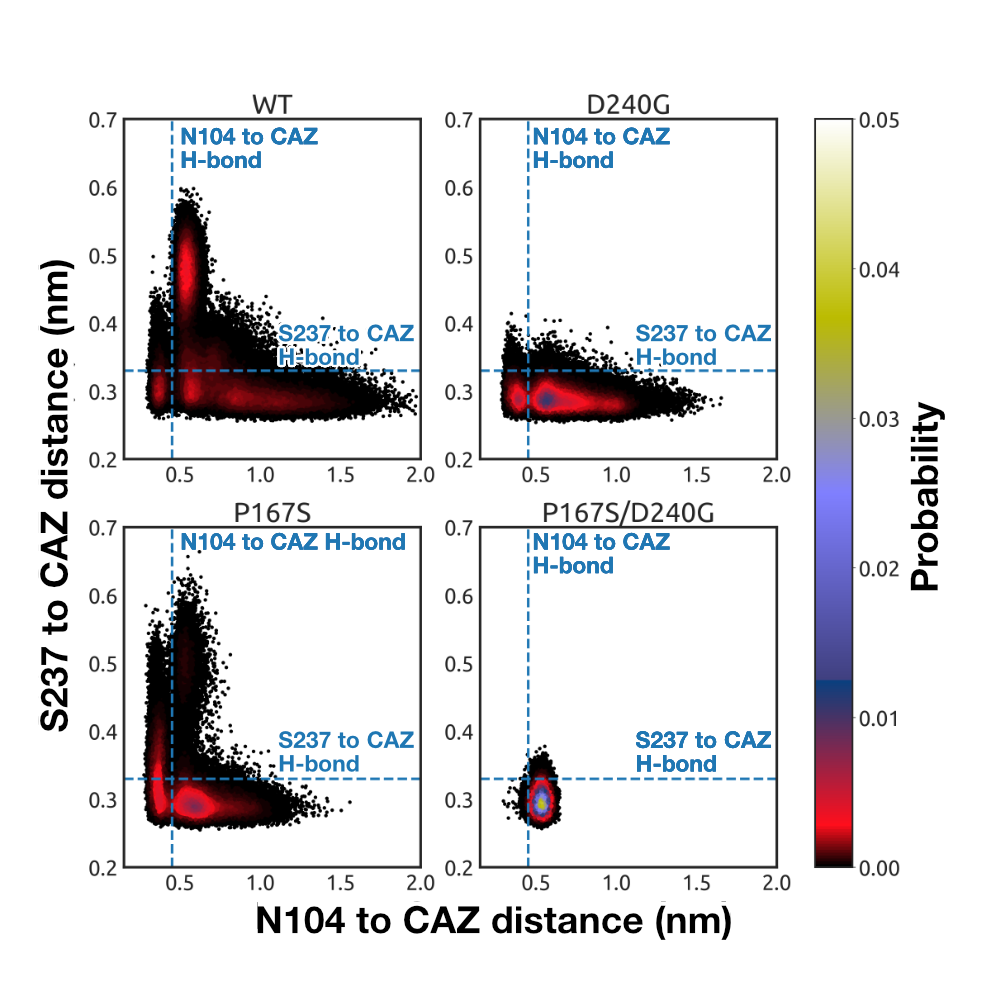
\includegraphics[width=5.5in]{ch2-suppfig1.png}
%             \caption[The $\beta$3 loop and Asn104 contact CAZ in the single mutants.]{The $\beta$3 loop and Asn104 contact CAZ in the single mutants. Joint distributions of two hydrogen-bonding distances that capture the contacts between CTX-M and ceftazidime (CAZ) in the acyl-enzyme complex: i) Asn104 to the imino group of ceftazidime and ii) the backbone nitrogen of S237 on the $\beta$3 loop to the $\beta$-Lactam carbonyl oxygen of ceftazidime. Distance cutoffs for hydrogen-bonding interactions are marked (dashed lines) to indicate whether or not an interaction occurs. Distributions are shown for wild type (top left), D240G (top right), P167S (bottom left), and P167S/D240G (bottom right). Each point represents a snapshot from the molecular dynamics simulations colored according to its probability based on a 2D histogram.}
%             \label{fig:ch2-suppfig1}
%         \end{figure} 

%         \begin{figure}[!htb] %Positioning code for figure
%             \centering
%             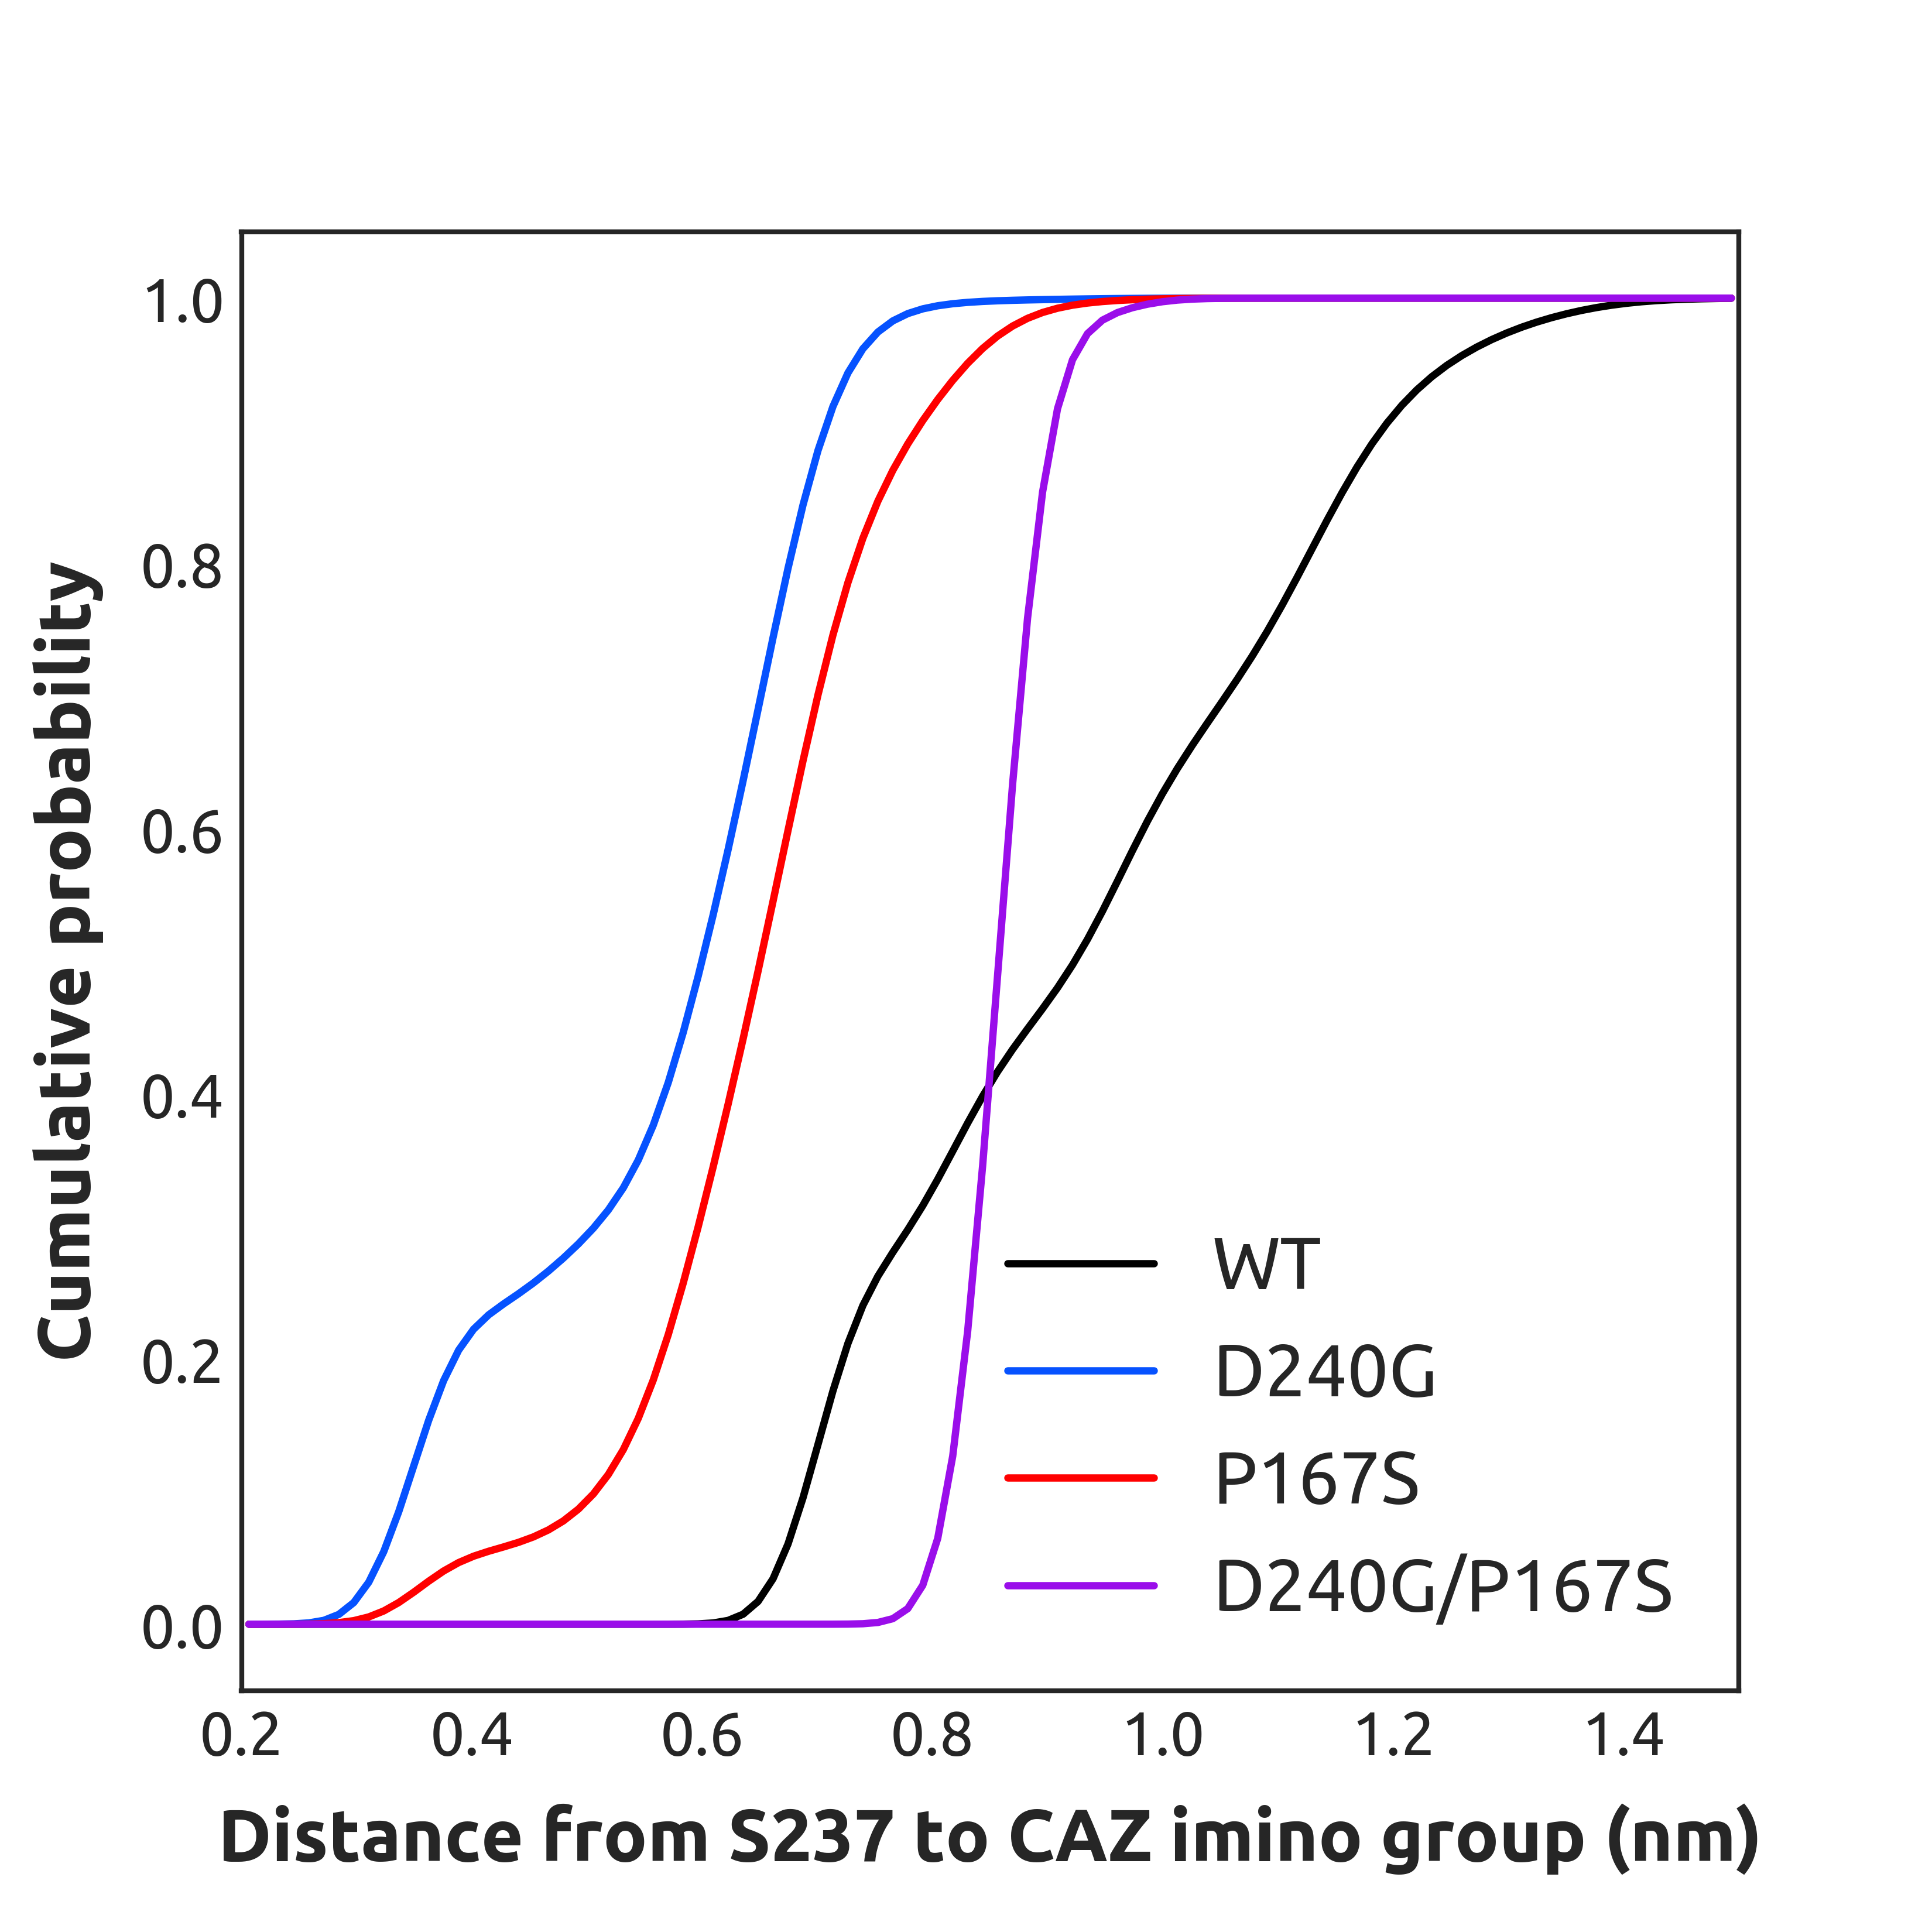
\includegraphics[width=5in]{ch2-suppfig2.png}
%             \caption[Ser237 makes contacts with the imino group of ceftazidime.]{Ser237 makes contacts with the imino group of ceftazidime. Cumulative distance distribution of the sidechain oxygen of Ser237 to the carboxylate of the imino group of ceftazdime in the acyl-enzyme complex. Distributions are shown for wild type (black), D240G (blue), P167S (red), and P167S/D240G (purple).}
%             \label{fig:ch2-suppfig2}
%         \end{figure} 

%         \begin{figure}[!htb] %Positioning code for figure
%             \centering
%             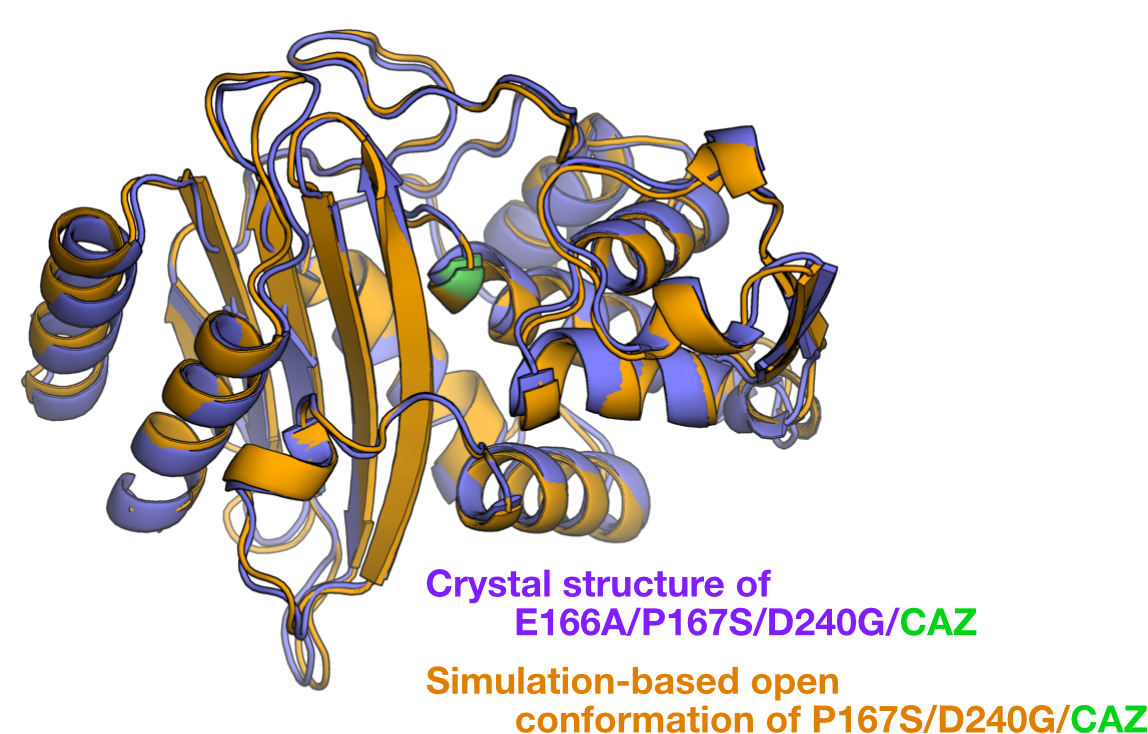
\includegraphics[width=5in]{ch2-suppfig3.png}
%             \caption[MD simulations of the closed conformation of P167S/D240G capture an open conformation of the $\Omega$-loop.]{MD simulations of the closed conformation of P167S/D240G capture an open conformation of the $\Omega$-loop. Overlay of the crystal structure of E166A/P167S/D240G/CAZ (purple, Ser70 colored in green) with a representative conformation from simulation of the open conformation of the $\Omega$-loop (orange, Ser70 colored in green) sampled from simulations of the P167S/D240G variant starting from the closed conformation. In both constructs the catalytic serine that forms the acyl-enzyme complex with the serine that binds ceftazidime (labelled CAZ) is colored green. The ceftazidime molecule is not shown for clarity.}
%             \label{fig:ch2-suppfig3}
%         \end{figure} 
    
    
   
%     % \% \section{Supplemental material}
%     % \%     \renewcommand{\thefigure}{\arabic{chapter}.S\arabic{figure}}
%     % \%     \setcounter{figure}{0}
%     % \%     \%Chapter 2 supplemental figures get labeled as Figure 2.S1 - 2.S(N). These still automatically pull into the List of Figures. You can do something similar for supplemental tables.
% \bibliography{../References}
% \bibliographystyle{unsrt}
\end{document}